The results are documented in this chapter.

The Python scripts used to calculate the statistical values and to plot the diagrams can be found in the
Appendix~\ref{sec:python_scripts}.

\subsection{Electrical Measurements}\label{sec:electrical_measurements}

This subchapter documents the measurement results that were recorded purely electrically (i.e. without the optical part.

The \acrfull{dso} used is a Rohde \& Schw arz RTB2004 1.25 GSa/s.

The time measurements are carried out by \lstinline|IC1| (see figure~\ref{fig:tdc_ele_signal}) and triggered and read by the
firmware, which is triggered and read on the Nucleo board \lstinline|U1| (see figure~\ref{fig:nucleo_board}).

\subsubsection{GPIO Toggle with HAL}\label{sec:gpio_toggle_with_hal}

First, the time it takes for the \acrshort{cpu} of the \acrshort{mcu} to switch two \acrshort{gpio} pins using the \acrfull{hal} library
\cite{st2020stm32f0_hal} is measured.

The firmware implementation for this is shown in Code~\ref{code:gpio_toggle_with_hal}.

\lstinputlisting[language={C}, label={code:gpio_toggle_with_hal}, caption={\acrshort{gpio} Toggle with \acrshort{hal}}]{../sourcecode/gpio_toggle_with_hal.c}

The \acrshort{tdc} measures the time between lines 15 and 16 in Code~\ref{code:gpio_toggle_with_hal}. To do this, the
STOP pin of the \acrshort{tdc} is connected to \lstinline|stop_ele| via \lstinline|SW1|. The cable connection \lstinline|J3|
is shorted. See figure~\ref{fig:tdc_ele_signal}.

Via \acrshort{uart}, 2000 measurement values were recorded. A section of this is shown in Code \ref{code:gpio_toggle_with_hal_log}.
The remaining data can be found in the electronic appendix.

\lstinputlisting[language={}, label={code:gpio_toggle_with_hal_log}, caption={\acrshort{gpio} Toggle with \acrshort{hal}}]{../sourcecode/gpio_toggle_with_hal_log.txt}

The arithmetic mean and standard deviation are listed in formula \ref{eq:gpio_toggle_with_hal}.

\begin{equation}\label{eq:gpio_toggle_with_hal}
      \begin{split}
            \overline{ToF} & = 6'375'888~ps \\
            \sigma         & = 1'059~ps
      \end{split}
\end{equation}
\myequations{\acrshort{gpio} Toggle with \acrshort{hal}}

Since the \acrshort{cpu} is running at 8~MHz, it can be concluded that a pin toggle with \acrshort{hal} takes about 50
\acrshort{cpu} cycles. This seems plausible.

The histogram and boxplot are shown in Figure~\ref{fig:gpio_toggle_with_hal_histogram} and
\ref{fig:gpio_toggle_with_hal_boxplot} shown.

\begin{figure}[H]
      \centering
      \includesvg[width=0.8\textwidth]{../graphics/gpio_toggle_with_hal_histogram.svg}
      \caption{\acrshort{gpio} Toggle with \acrshort{hal} - Histogram}\label{fig:gpio_toggle_with_hal_histogram}
\end{figure}

\begin{figure}[H]
      \centering
      \includesvg[width=0.8\textwidth]{../graphics/gpio_toggle_with_hal_boxplot.svg}
      \caption{\acrshort{gpio} Toggle with \acrshort{hal} - Boxplot}\label{fig:gpio_toggle_with_hal_boxplot}
\end{figure}

To validate the results of the \acrshort{tdc}, the same measurement was also carried out using \acrfull{dso}. The
measurements are shown in Figure~\ref{fig:gpio_toggle_with_hal_dso} and \ref{fig:gpio_toggle_with_hal_dso_zoom}.

\begin{figure}[H]
      \centering
      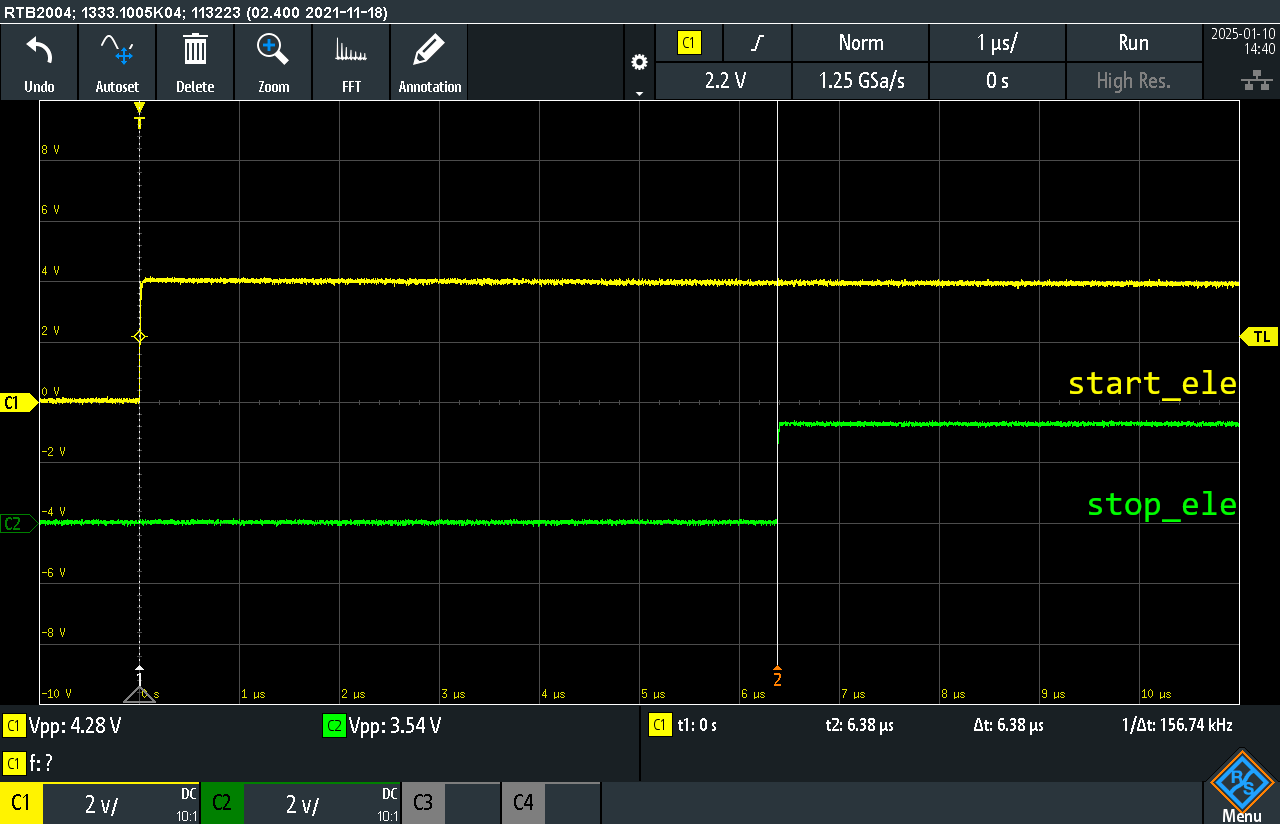
\includegraphics[width=0.8\textwidth]{../graphics/gpio_toggle_with_hal_dso.png}
      \caption{\acrshort{gpio} Toggle with \acrshort{hal} - \acrshort{dso}}\label{fig:gpio_toggle_with_hal_dso}
\end{figure}

\begin{figure}[H]
      \centering
      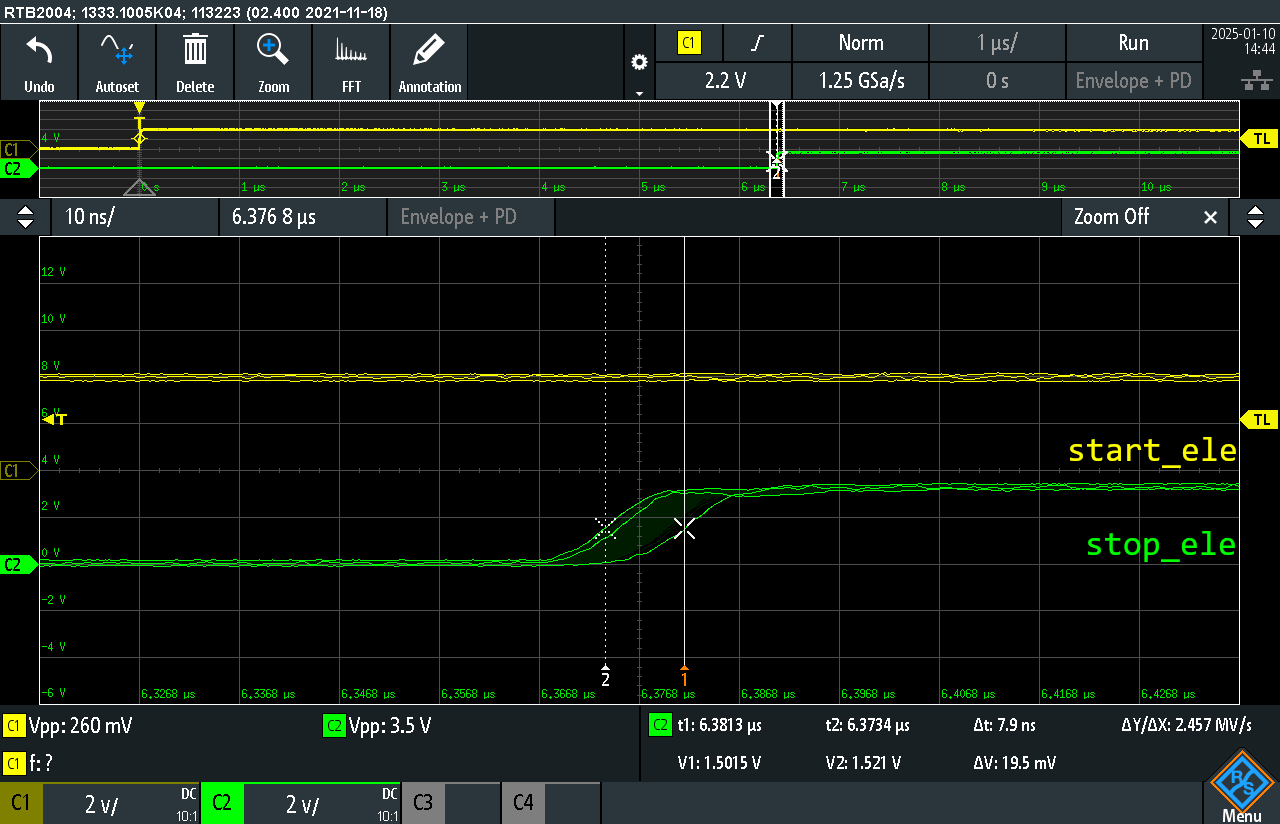
\includegraphics[width=0.8\textwidth]{../graphics/gpio_toggle_with_hal_dso_zoom.png}
      \caption{\acrshort{gpio} Toggle with \acrshort{hal} - \acrshort{dso} (Zoom)}\label{fig:gpio_toggle_with_hal_dso_zoom}
\end{figure}

\subsubsection{GPIO Toggle without HAL}\label{sec:gpio_toggle_without_hal}

Next, we measure how long it takes for the \acrshort{cpu} of the \acrshort{mcu} to switch two \acrshort{gpio} pins using direct register access
(via pointer; without \acrshort{hal} library).

The firmware implementation for this is shown in Code~\ref{code:gpio_toggle_without_hal}.

\lstinputlisting[language={C}, label={code:gpio_toggle_without_hal}, caption={\acrshort{gpio} Toggle without \acrshort{hal}}]{../sourcecode/gpio_toggle_without_hal.c}

The \acrshort{tdc} thus measures the time between lines 15 and 16 in Code~\ref{code:gpio_toggle_without_hal}. To do this,
as in chapter \ref{sec:gpio_toggle_with_hal}, the STOP pin of the \acrshort{tdc} is connected to \lstinline|SW1| via \lstinline|SW1|
\lstinline|stop_ele|. The cable connection \lstinline|J3| is shorted. See
Figure~\ref{fig:tdc_ele_signal}.

Via \acrshort{uart}, 2000 measurement values were recorded. A section of this is shown in Code
\ref{code:gpio_toggle_without_hal_log} shown. The remaining data can be found in the electronic appendix.

\lstinputlisting[language={}, label={code:gpio_toggle_without_hal_log}, caption={\acrshort{gpio} Toggle ohne \acrshort{hal}}]{../sourcecode/gpio_toggle_without_hal_log.txt}

The arithmetic mean and standard deviation are listed in formula \ref{eq:gpio_toggle_without_hal}.

\begin{equation}\label{eq:gpio_toggle_without_hal}
      \begin{split}
            \overline{ToF} & = 1'377'773~ps \\
            \sigma         & = 402~ps
      \end{split}
\end{equation}
\myequations{\acrshort{gpio} Toggle without \acrshort{hal}}

Since the \acrshort{cpu} is running at 8~MHz, it can be concluded that a pin toggle without \acrshort{hal} takes about 10
\acrshort{cpu} cycles. This seems plausible.

The histogram and boxplot are shown in figures~\ref{fig:gpio_toggle_without_hal_histogram} and
\ref{fig:gpio_toggle_without_hal_boxplot}, respectively.

\begin{figure}[H]
      \centering
      \includesvg[width=0.8\textwidth]{../graphics/gpio_toggle_without_hal_histogram.svg}
      \caption{\acrshort{gpio} Toggle without \acrshort{hal} - Histogram}\label{fig:gpio_toggle_without_hal_histogram}
\end{figure}

\begin{figure}[H]
      \centering
      \includesvg[width=0.8\textwidth]{../graphics/gpio_toggle_without_hal_boxplot.svg}
      \caption{\acrshort{gpio} Toggle without \acrshort{hal} - Boxplot}\label{fig:gpio_toggle_without_hal_boxplot}
\end{figure}

To validate the results of the \acrshort{tdc}, the same measurement was also carried out using \acrfull{dso}. The
measurements are shown in Figure~\ref{fig:gpio_toggle_without_hal_dso} and \ref{fig:gpio_toggle_without_hal_dso_zoom}.

\begin{figure}[H]
      \centering
      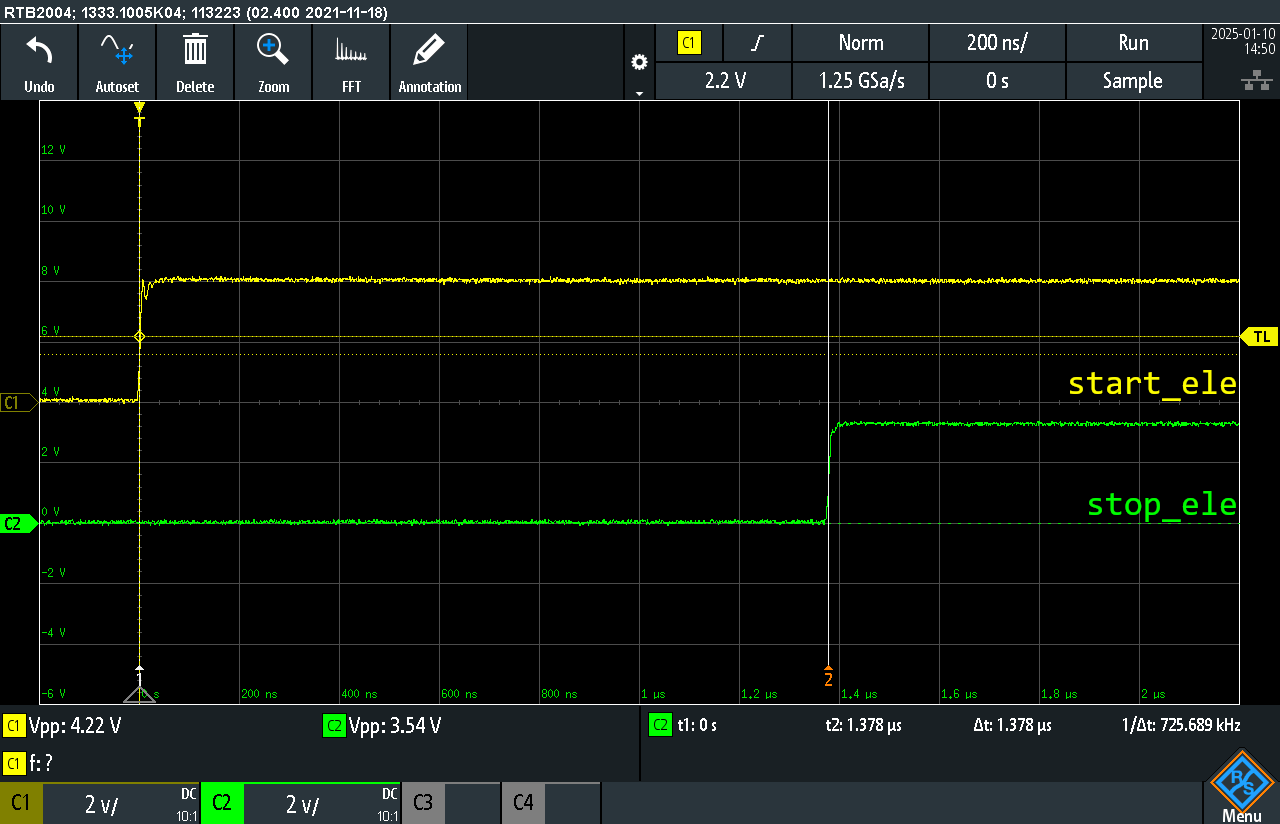
\includegraphics[width=0.8\textwidth]{../graphics/gpio_toggle_without_hal_dso.png}
      \caption{\acrshort{gpio} Toggle without \acrshort{hal} - \acrshort{dso}}\label{fig:gpio_toggle_without_hal_dso}
\end{figure}

\begin{figure}[H]
      \centering
      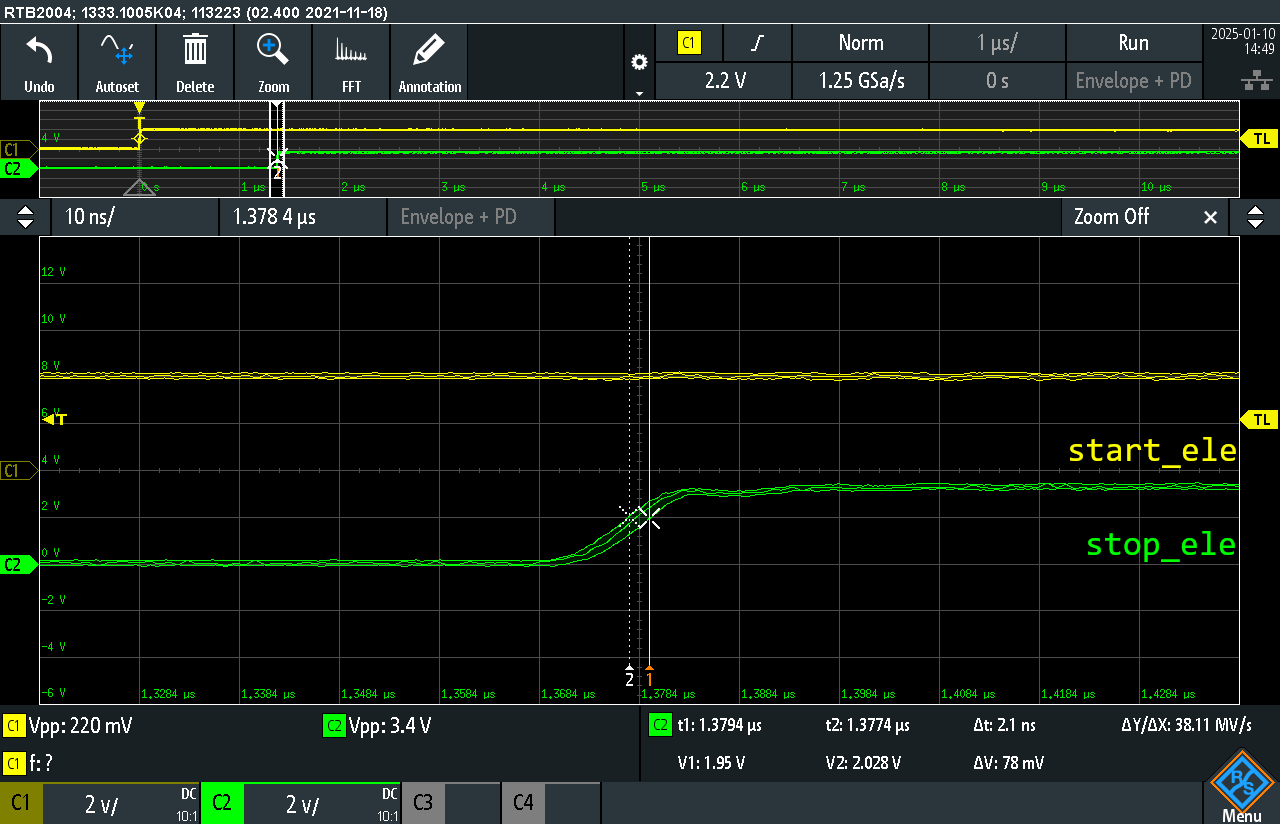
\includegraphics[width=0.8\textwidth]{../graphics/gpio_toggle_without_hal_dso_zoom.png}
      \caption{\acrshort{gpio} Toggle without \acrshort{hal} - \acrshort{dso} (Zoom)}\label{fig:gpio_toggle_without_hal_dso_zoom}
\end{figure}

\subsubsection{Different cable lengths}\label{sec:different_cable_lengths}

For this measurement, the same setup as in chapter \ref{sec:gpio_toggle_without_hal} is used.

Instead of short-circuiting \lstinline|J3| (see figure \ref{fig:tdc_ele_signal}), different cable lengths are now
connected.

A single insulated copper wire ($\diameter_{cu} = 0.8~mm$, $\diameter_{ges} = 1.6~mm$) is used as the cable.

It has been found that a circular arrangement of the cable is important. This is because when the
the two cable ends overlap, short times are measured. This has to do with the capacitive coupling between the conductors.

The results are shown in Figure~\ref{fig:different_cable_lengths}. The list with the data points
can be found in the electronic appendix.

\begin{figure}[H]
      \centering
      \includesvg[width=0.9\textwidth]{../graphics/different_cable_lengths.svg}
      \caption{Different cable lengths}\label{fig:different_cable_lengths}
\end{figure}

The arithmetic mean values and standard deviations are listed in Table \ref{tab:different_cable_lengths}.

\begin{table}[H]
      \mytable
      {|l|l|l|}
      {\textbf{Length} & \textbf{Mean value} & \textbf{Standard deviation}}
      {\length & \mean & \stddev}
      {../tables/different_cable_lengths.csv}
      \caption{Different cable lengths}\label{tab:different_cable_lengths}
\end{table}

The signal propagation speed in copper is approximately $\sfrac{2}{3}$ of the speed of light
\cite{firewallcx2025propagationdelay}. To validate the results in Table \ref{tab:different_cable_lengths},
we calculate back to the cable length, as shown in formula \ref{eq:cable_length}. The runtime at 0~m is
subtracted to compensate for the delay caused by switching the \acrshort{gpio}s.

\begin{equation}\label{eq:cable_length}
      \begin{split}
            c_{cu}  & \approx \frac{2}{3} \cdot c_0 = \frac{2}{3} \cdot 299'792'458~\frac{m}{s} \approx 200'000'000~\frac{m}{s} \\
            ToF_{n} & = ToF_{n_{abs}} - ToF_{0}                                                                                 \\
            l_{n}   & = ToF_{n} \cdot c_{cu}
      \end{split}
\end{equation}
\myequations{Back-calculate to cable length}

The results are shown in Table \ref{tab:different_cable_lengths_calc}.

\begin{table}[H]
      \mytable
      {|l|l|l|}
      {\textbf{Actual length} & \textbf{ToF}$\mathbf{_n}$ & \textbf{Calculated length}}
      {\reallength & \tofn & \calclength}
      {../tables/different_cable_lengths_calc.csv}
      \caption{Calculated cable lengths}\label{tab:different_cable_lengths_calc}
\end{table}

It is noticeable that the results do not match exactly. However, a clear correlation can be seen.

The difference could have various causes. One possible explanation would be that the propagation speed
of the cable used is closer to the speed of light than assumed. Further measurement results and evaluations
in chapter~\ref{sec:different_cable_lengths_with_dso}.

\subsubsection{Mode 1 vs. Mode 2}

The TDC7200 supports two modes with different measurement ranges \cite{ti2016tdc7200_datasheet}:

\begin{itemize}
      \item Mode 1: 12~ns to 500~ns
      \item Mode 2: 250~ns to 8~ms
\end{itemize}

In mode 1, only the internal ring oscillator of the \acrshort{tdc} is used. See figure~\ref{fig:tdc_mode1}.

\begin{figure}[H]
      \centering
      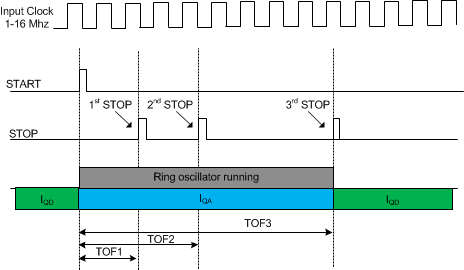
\includegraphics[width=0.6\textwidth]{../graphics/tdc_mode1.png}
      \caption[\acrshort{tdc} Mode 1]{\acrshort{tdc} Mode 1 \cite{ti2016tdc7200_datasheet}}\label{fig:tdc_mode1}
\end{figure}

In mode 2, to be able to measure longer times, the external clock of the \acrshort{tdc} is also used. See
Figure~\ref{fig:tdc_mode2}.

\begin{figure}[H]
      \centering
      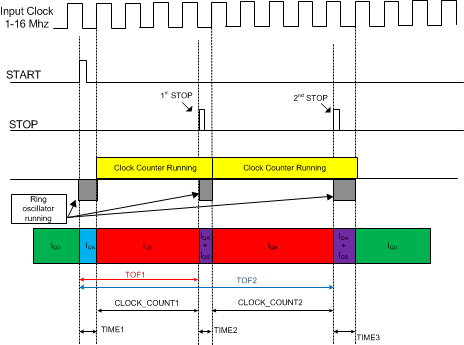
\includegraphics[width=0.6\textwidth]{../graphics/tdc_mode2.png}
      \caption[\acrshort{tdc} Mode 2]{\acrshort{tdc} Mode 2 \cite{ti2016tdc7200_datasheet}}\label{fig:tdc_mode2}
\end{figure}

The previous measurements (chapter~\ref{sec:gpio_toggle_with_hal}, \ref{sec:gpio_toggle_without_hal} and
\ref{sec:different_cable_lengths}) were performed in mode~2 because switching the \acrshort{gpio}s with the
\acrshort{cpu} took more than 500~ns.

In future measurements, the \acrshort{gpio}s are to be switched by a hardware timer of the \acrshort{mcu}.
This will enable switching times of 125 ns at 8 MHz and 20.8 ns at 48 MHz. This chapter will therefore
compare the measurement results of the two modes.

Three measurements were made for this purpose:

\begin{enumerate}
      \item \acrshort{gpio} Toggle without \acrshort{hal} in mode 2 with cable length = 0 m (as in chapter \ref{sec:gpio_toggle_without_hal} and \ref{sec:different_cable_lengths})
      \item \acrshort{gpio} Toggle without \acrshort{hal} in mode 2 with cable length 6 m (as in chapter \ref{sec:different_cable_lengths})
      \item Without GPIO Toggle in mode 1 with cable length 6 m
\end{enumerate}

For the measurement in mode 1, the delay caused by switching the \acrshort{gpio}s should be avoided. To do this,
the \lstinline|START| and \lstinline|STOP| signals are generated by the same \acrshort{gpio} pin, \lstinline|start_ele|.
To do this, \lstinline|SW1| is connected to \lstinline|start_ele| (see figure~\ref{fig:tdc_ele_signal}).

The firmware implementation for a measurement in mode~1 is shown in code~\ref{code:mode1}.

\lstinputlisting[language={C}, label={code:mode1}, caption={Mode 1}]{../sourcecode/mode1.c}

The differences compared to the measurements in chapter~\ref{sec:gpio_toggle_without_hal} and
\ref{sec:different_cable_lengths} are:

\begin{itemize}
      \item Line 7: \acrshort{tdc} is configured in mode 1 (instead of mode 2)
      \item Line 15 and 23: Only the \lstinline|start_ele| pin is toggled (instead of the \lstinline|start_ele| and \lstinline|stop_ele| pins)
\end{itemize}

The expectation is that the difference between measurement~1 and measurements~2 roughly corresponds to the result of
measurement~3.

The results of these three measurements are listed in Table \ref{tab:mode1_vs_mode2}. The remaining data can be found
in the electronic appendix.

\begin{table}[H]
      \mytable
      {|l|l|l|}
      {\textbf{Measurement} & \textbf{Mean value} & \textbf{Standard deviation}}
      {\measurement & \mean & \stddev}
      {../tables/mode1_vs_mode2.csv}
      \caption{Mode 1 vs. Mode 2}\label{tab:mode1_vs_mode2}
\end{table}

The calculation in formula~\ref{eq:mode1_vs_mode2} shows that the measurement results are close.

\begin{equation}\label{eq:mode1_vs_mode2}
      \begin{split}
            \Delta Mode~2 & = 1'403'224~ps - 1'378'222~ps = 25'001~ps \\
            Mode~1        & = 25'145 ps
      \end{split}
\end{equation}
\myequations{Mode 1 vs. Mode 2}

It can be assumed that Mode~1 and Mode~2 have been correctly implemented in the firmware driver.

Note: In the firmware driver (see appendix~\ref{sec:tdc_driver}), the same function can be used for both modes
\lstinline|TDC_read_result()|. For mode~1, the calculation is simplified because \lstinline|TIME2|~=~0 and
\lstinline|CLOCK_COUNT1|~=~0.

\subsubsection{Timer Output}\label{sec:timer_output}

In chapters~\ref{sec:gpio_toggle_with_hal} and \ref{sec:gpio_toggle_without_hal} it was shown that it takes several
\acrshort{cpu} cycles to toggle \acrshort{gpio}s using software, i.e. \acrshort{cpu} instructions.

A faster method is to have the \acrshort{gpio}s toggled by the \acrshort{mcu}'s hardware peripherals. Hardware timers
are suitable for this purpose.

Figure \ref{fig:clock_config_default} shows the default clock configuration of the Nucleo board.

\begin{figure}[H]
      \centering
      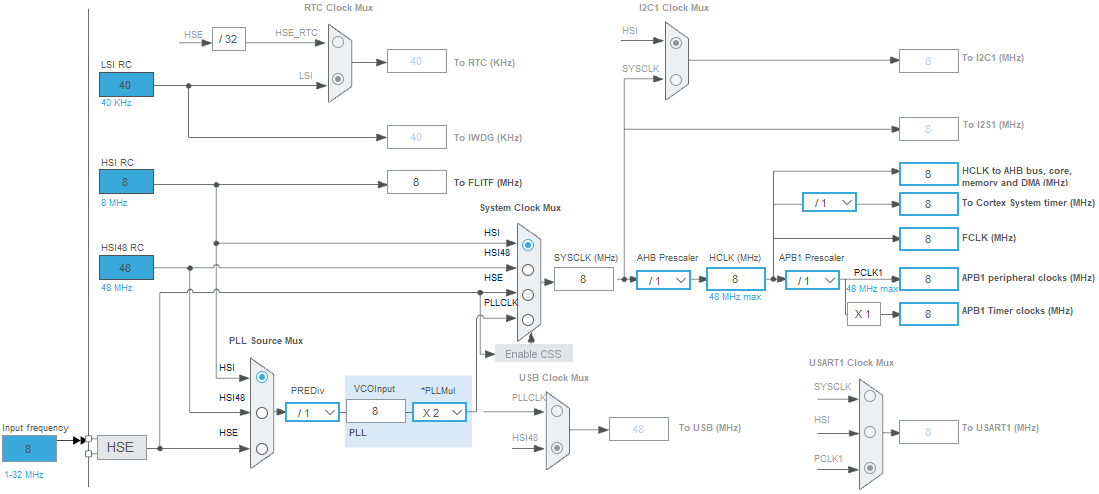
\includegraphics[width=0.9\textwidth]{../graphics/clock_config_default.png}
      \caption{Default clock configuration}\label{fig:clock_config_default}
\end{figure}

By default, the \acrfull{hsi} clock is used at 8~MHz. This should make it possible to use the hardware timer to switch two
\acrshort{gpio}s with a delay according to the formula~\ref{eq:gpio_schalten_zeit}.

\begin{equation}\label{eq:gpio_schalten_zeit}
      t = \frac{1}{8~MHz} = 125~ns
\end{equation}
\myequations{\acrshort{gpio}-switching delay time}

For this purpose, channels \lstinline|CH1| and \lstinline|CH4| of the hardware timer \lstinline|TIM1| are used in Output Compare Match mode.
The associated \acrshort{gpio} pins are \lstinline|start_ele| and \lstinline|stop_ele|, respectively.

When the 16-bit timer reaches \lstinline|32'000|, \lstinline|start_ele| is switched to high. When the
value \lstinline|32'001| is reached, \lstinline|stop_ele| is switched to high.

The \acrshort{tdc} is configured in mode 1. The STOP pin of the \acrshort{tdc} is connected to \lstinline|SW1| via
\lstinline|stop_ele|. The cable connection \lstinline|J3| is shorted. See
Figure~\ref{fig:tdc_ele_signal}.

The firmware implementation for this is shown in Code~\ref{code:timer_output}.

\lstinputlisting[language={C}, label={code:timer_output}, caption={\acrshort{gpio} Toggle with timer output}]{../sourcecode/timer_output.c}

The measured arithmetic mean and standard deviation are listed in formula~\ref{eq:timer_output}. The list of data points
can be found in the electronic appendix.

\begin{equation}\label{eq:timer_output}
      \begin{split}
            \overline{ToF} & =128'108~ps \\
            \sigma         & = 81~ps
      \end{split}
\end{equation}
\myequations{\acrshort{gpio} Toggle with timer output}

As expected, switching the \acrshort{gpio}s takes about 125 ns. The standard deviation is lower than in the previous chapters due to the smaller
number of clock cycles.

\subsubsection{Different Clock Configurations}

In this subsection, measurements are performed with the same setup as in chapter~\ref{sec:timer_output}.

The arithmetic mean values and standard deviations of different clock sources of the Nucleo board are compared.
Three measurements are made:

\begin{enumerate}
      \item \acrshort{hsi}: 8~MHz (as in chapter~\ref{sec:timer_output})
      \item \acrshort{hsi} with \acrshort{pll}: 16~MHz
      \item \acrshort{hsi}48: 48~MHz
\end{enumerate}

The clock configurations for measurements 2 and 3 are shown in Figure~\ref{fig:clock_config_hsi_pll_16mhz} and
\ref{fig:clock_config_hsi48_48mhz}, respectively.

\begin{figure}[H]
      \centering
      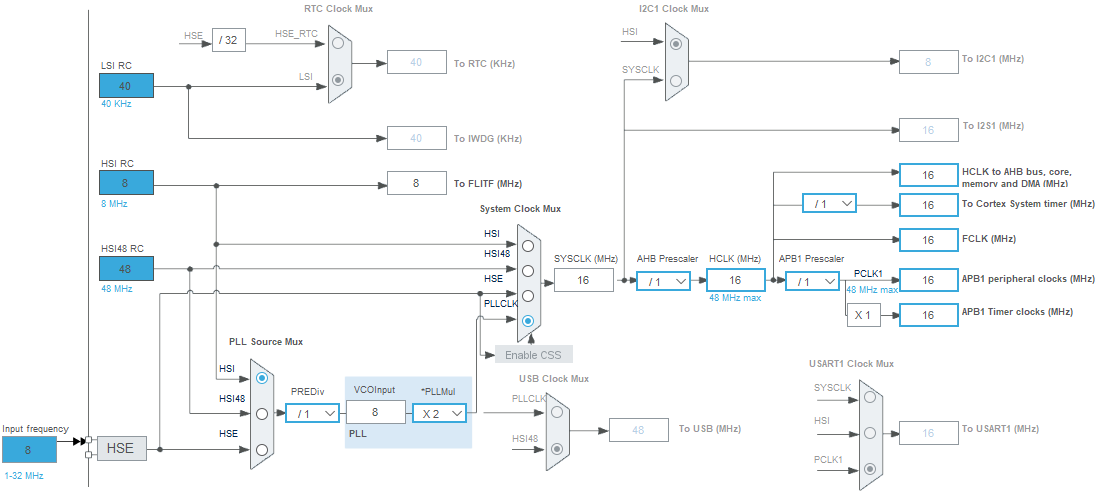
\includegraphics[width=0.9\textwidth]{../graphics/clock_config_hsi_pll_16mhz.png}
      \caption{Clock configuration \acrshort{hsi} with \acrshort{pll} 16~MHz}\label{fig:clock_config_hsi_pll_16mhz}
\end{figure}

\begin{figure}[H]
      \centering
      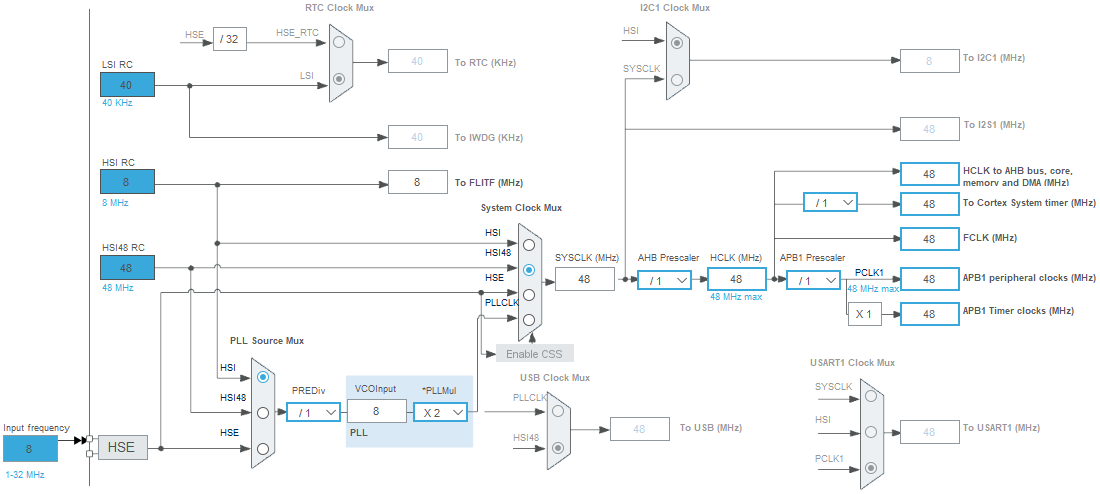
\includegraphics[width=0.9\textwidth]{../graphics/clock_config_hsi48_48mhz.png}
      \caption{Clock configuration \acrshort{hsi}48 48~MHz}\label{fig:clock_config_hsi48_48mhz}
\end{figure}

The arithmetic mean values and standard deviations are shown in Table~\ref{tab:different_clock_sources}.
The list of data points can be found in the electronic appendix.

\begin{table}[H]
      \mytable
      {|l|l|l|}
      {\textbf{Measurement} & \textbf{Mean value} & \textbf{Standard deviation}}
      {\measurement & \mean & \stddev}
      {../tables/different_clock_sources.csv}
      \caption{Different clock sources}\label{tab:different_clock_sources}
\end{table}

The results roughly match the expected values from formula~\ref{eq:gpio_schalten_zeiten}.

\begin{equation}\label{eq:gpio_schalten_zeiten}
      \begin{split}
            t_1 & = \frac{1}{8~MHz} = 125~ns   \\
            t_2 & = \frac{1}{16~MHz} = 62.5~ns \\
            t_3 & = \frac{1}{48~MHz} = 20.8~ns
      \end{split}
\end{equation}
\myequations{\acrshort{gpio}-switching delay times}

The data sheet contains information about the \acrshort{pll} jitter, see figure~\ref{fig:pll_jitter}.

\begin{figure}[H]
      \centering
      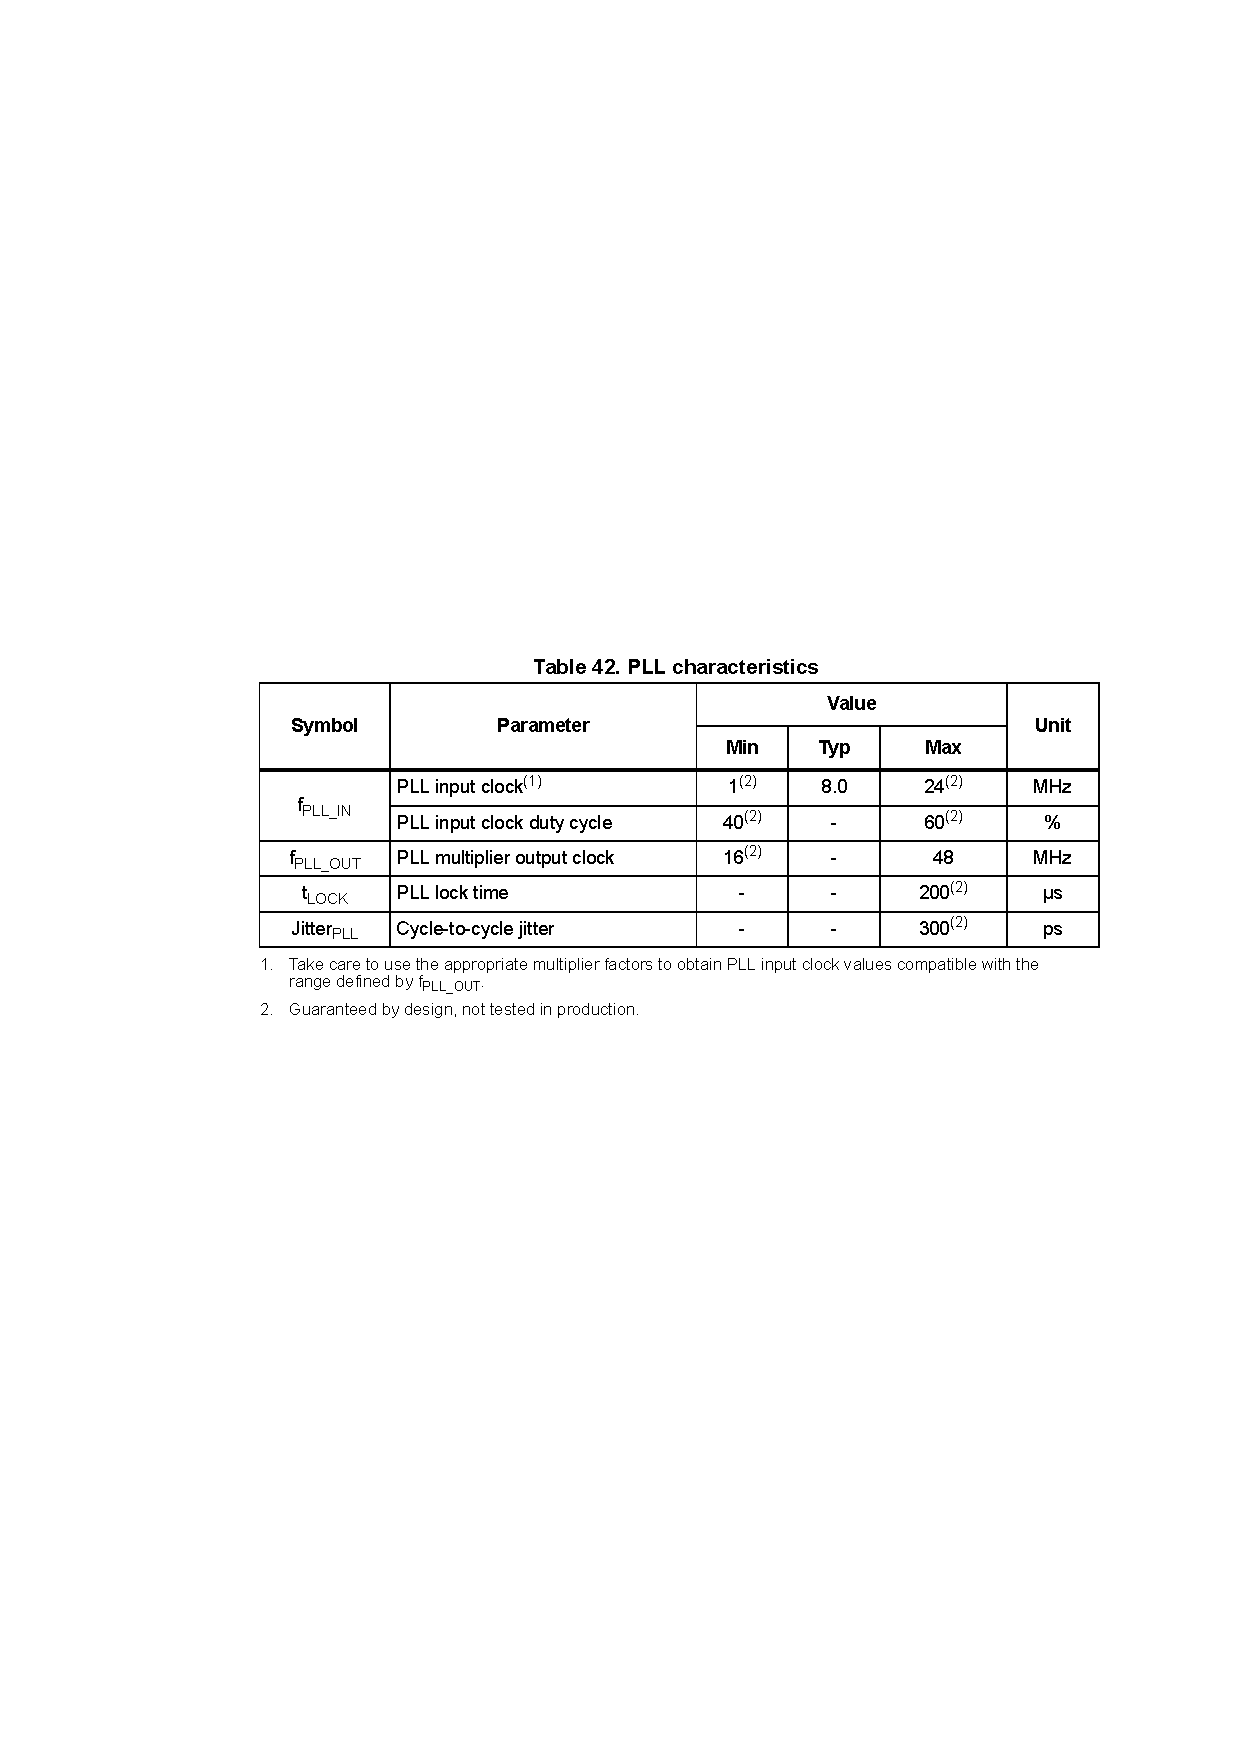
\includegraphics[width=0.8\textwidth]{../graphics/pll_jitter.pdf}
      \caption[\acrshort{pll}-Jitter]{\acrshort{pll}-Jitter \cite{st2017stm32f042k6_datasheet}}\label{fig:pll_jitter}
\end{figure}

This information is approximately in the same order of magnitude as the measurement results.

\subsubsection{Different cable lengths with DSO}\label{sec:different_cable_lengths_with_dso}

In this subchapter, the same cable lengths as in chapter~\ref{sec:different_cable_lengths}
are measured again.

The following firmware configuration is used to reduce the jitter:

\begin{itemize}
      \item \acrshort{tdc}: Mode 1
      \item Clock: 48~MHz
      \item Switching the \acrshort{gpio}s: Timer Output
\end{itemize}

In addition, the different cable lengths are also measured simultaneously via \acrshort{dso} (Rohde \& Schwarz RTB2004
2.5 GSa/s.) in order to compare the results of the \acrshort{tdc} with them.

Figure~\ref{fig:different_cable_lengths_with_dso_tdc} shows the recorded measurement results of the \acrshort{tdc}.
While the measurement values were being recorded, the \acrshort{dso} was connected to the pins. The list of
data points can be found in the electronic appendix.

\begin{figure}[H]
      \centering
      \includesvg[width=0.9\textwidth]{../graphics/different_cable_lengths_with_dso_tdc.svg}
      \caption{Different cable lengths - measurement values \acrshort{tdc}}\label{fig:different_cable_lengths_with_dso_tdc}
\end{figure}

Table~\ref{tab:different_cable_lengths_with_dso_tdc} lists the mean values and standard deviations of the
measured results of the \acrshort{tdc}.

\begin{table}[H]
      \mytable
      {|l|l|l|l|}
      {\textbf{Length} & \textbf{Mean value} & \textbf{Standard deviation} & \textbf{$\Delta$ at 0~m}}
      {\length & \mean & \stddev & \diff}
      {../tables/different_cable_lengths_with_dso_tdc.csv}
      \caption{Different cable lengths - results \acrshort{tdc}}\label{tab:different_cable_lengths_with_dso_tdc}
\end{table}

The measurement results recorded by the \acrshort{dso} are listed in Table~\ref{tab:different_cable_lengths_with_dso_dso}.
The last column shows the difference between \acrshort{dso} and \acrshort{tdc}. It can be seen that the difference is
very small.

\begin{table}[H]
      \mytable
      {|l|l|l|l|}
      {\textbf{Length} & \textbf{Value} & \textbf{$\Delta$ at 0~m} & \textbf{$\Delta$ at TDC}}
      {\length & \measurement & \diff & \difftdc}
      {../tables/different_cable_lengths_with_dso_dso.csv}
      \caption{Different cable lengths - results \acrshort{dso}}\label{tab:different_cable_lengths_with_dso_dso}
\end{table}

Table~\ref{tab:different_cable_lengths_with_dso_theorie} shows the theoretically expected propagation times for the
different assumptions for the signal propagation velocities of $\sfrac{2}{3}~c$ and $c$.

\begin{table}[H]
      \mytable
      {|l|l|l|}
      {\textbf{Length} & \textbf{Theory} $\mathbf{\sfrac{2}{3}~c}$ & \textbf{Theory c}}
      {\length & \theoriekc & \theoriec}
      {../tables/different_cable_lengths_with_dso_theorie.csv}
      \caption{Different cable lengths - theoretical expectation}\label{tab:different_cable_lengths_with_dso_theorie}
\end{table}

The differences between the \acrshort{tdc} results and the theoretical expectations are shown in the
tables~\ref{tab:different_cable_lengths_with_dso_theorie_vs_tdc_ns} and
\ref{tab:different_cable_lengths_with_dso_theorie_vs_tdc_m}. First, the difference in runtime is shown,
then the recalculated cable length.

\begin{table}[H]
      \mytable
      {|l|l|l|}
      {\textbf{Length} & \textbf{$\Delta$ TDC to theory} $\mathbf{\sfrac{2}{3}~c}$ & \textbf{$\Delta$ TDC theory to c}}
      {\length & \tdczutheoriekc & \tdczutheoriec}
      {../tables/different_cable_lengths_with_dso_theorie_vs_tdc_ns.csv}
      \caption{Different cable lengths - \acrshort{tdc}[ns] difference compared to theory}\label{tab:different_cable_lengths_with_dso_theorie_vs_tdc_ns}
\end{table}

\begin{table}[H]
      \mytable
      {|l|l|l|}
      {\textbf{Length} & \textbf{TDC acc. to theory} $\mathbf{\sfrac{2}{3}~c}$ & \textbf{TDC acc. to theory c}}
      {\length & \tdcgemtheoriekc & \tdcgemtheoriec}
      {../tables/different_cable_lengths_with_dso_theorie_vs_tdc_m.csv}
      \caption{Different cable lengths - \acrshort{tdc} [m] according to theory}\label{tab:different_cable_lengths_with_dso_theorie_vs_tdc_m}
\end{table}

Table~\ref{tab:different_cable_lengths_with_dso_theorie_vs_tdc_m} shows that neither of the two
theoretical values for $c$ lead to a perfect \acrshort{tdc} result for the recalculated distance [m].

In Table~\ref{tab:different_cable_lengths_with_dso_theorie_vs_tdc_ns}, we see that the difference between the
\acrshort{tdc} results compared to the theoretically expected runtime at $c$ is slightly smaller than at $\sfrac{2}{3}~c$. It
seems that $c$ is a slightly better approximation.

If the measured difference can actually be explained by an incorrect assumption of the propagation speed, then the
propagation speed in the selected cable would have to be approximately $0.9~c$. The recalculated results are listed in
Table~\ref{tab:different_cable_lengths_with_dso_theorie09_vs_tdc_m}.

\begin{table}[H]
      \mytable
      {|l|l|}
      {\textbf{Length} & \textbf{TDC acc. to theory 0.9 c}}
      {\length & \tdcgemtheoriemc}
      {../tables/different_cable_lengths_with_dso_theorie09_vs_tdc_m.csv}
      \caption{Different cable lengths - \acrshort{tdc} [m] according to the 0.9 c theory}\label{tab:different_cable_lengths_with_dso_theorie09_vs_tdc_m}
\end{table}

The figures~\ref{fig:different_cable_lengths_with_dso_1m} and \ref{fig:different_cable_lengths_with_dso_6m} show
the \acrshort{dso} records for cable lengths of 1~m and 6~m are shown. The remaining \acrshort{dso} records
can be found in the electronic appendix.

\begin{figure}[H]
      \centering
      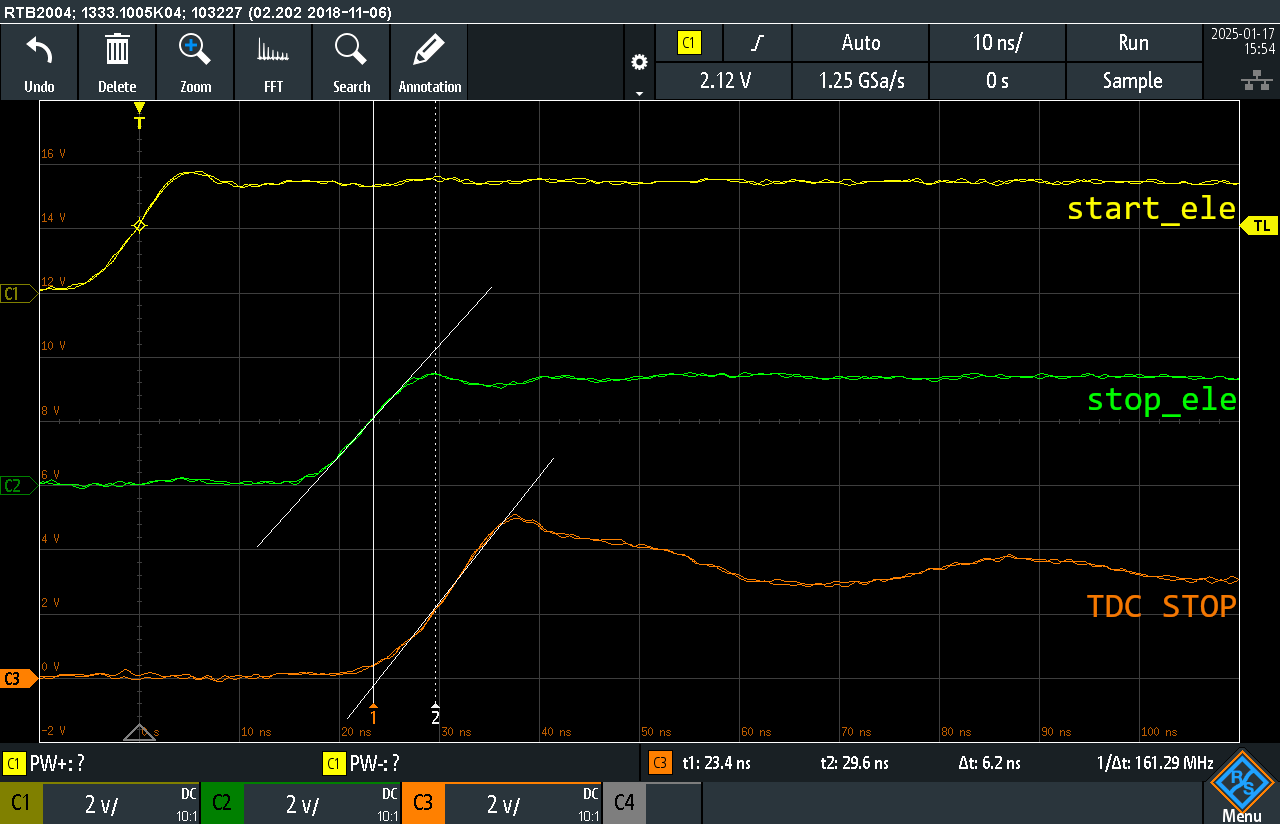
\includegraphics[width=\textwidth]{../graphics/different_cable_lengths_with_dso_1m.png}
      \caption{\acrshort{dso} recording with a cable length of 1~m}\label{fig:different_cable_lengths_with_dso_1m}
\end{figure}

\begin{figure}[H]
      \centering
      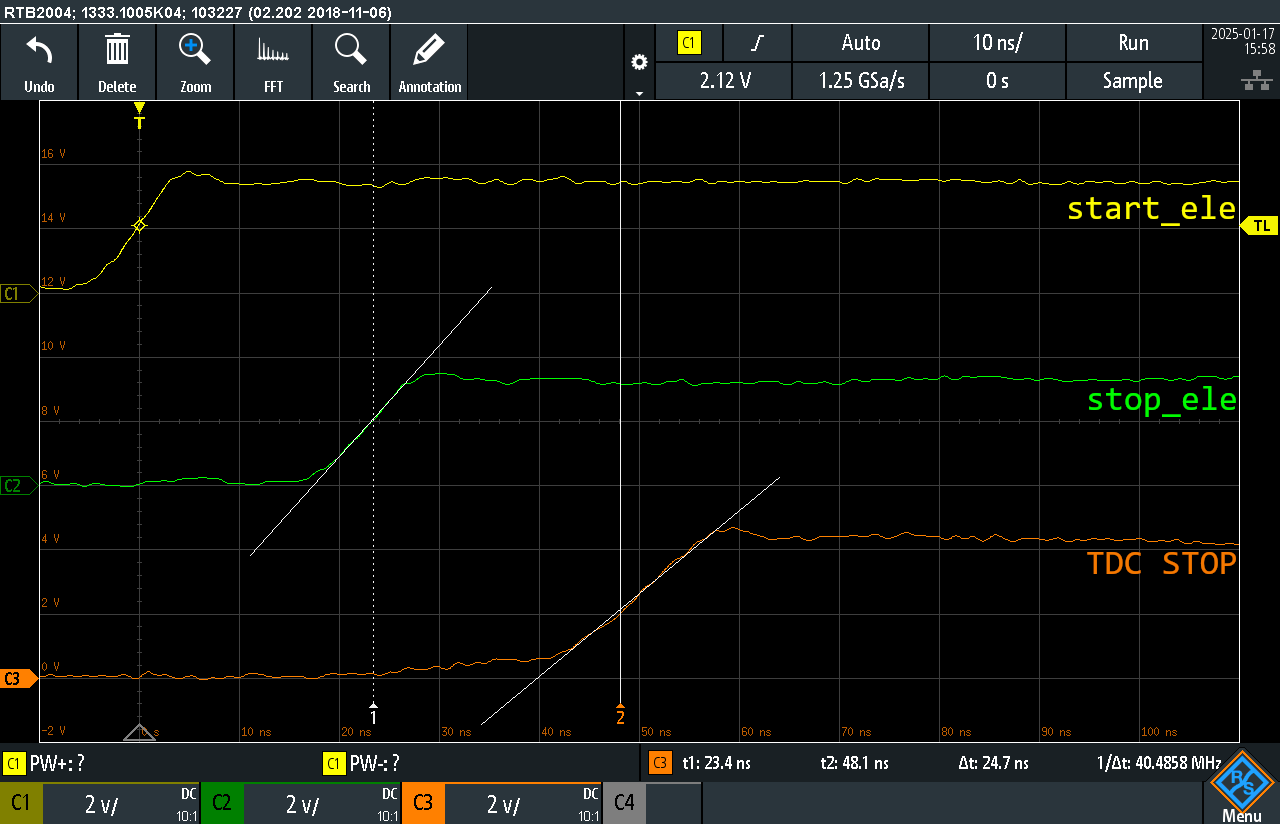
\includegraphics[width=\textwidth]{../graphics/different_cable_lengths_with_dso_6m.png}
      \caption{\acrshort{dso} recording with a cable length of 6 m}\label{fig:different_cable_lengths_with_dso_6m}
\end{figure}

It can be seen that the slope of the \lstinline|STOP| signal flattens out a little with longer cable lengths. This has an
influence on the runtime measurement. Steeper edges would help to minimize this influence. More about this in
chapter~\ref{sec:ausblick}.

\pagebreak

\subsection{Optical Measurements}
This subsection documents the measurement results that relate to the optical path of the demonstrator.

The \acrshort{dso} used is a Rohde \& Schwarz RTB2004 2.5 GSa/s.

The following firmware configurations are used for the measurements in this chapter:

\begin{itemize}
      \item \acrshort{tdc}: Mode 1
      \item Clock: 48~MHz
      \item Switching the \acrshort{gpio}s: Timer Output
\end{itemize}

\subsubsection{Signal Path Transmitter}\label{sec:messungen_signalpfad_sender}

In this subsection, the signal path of the optical transmitter is measured.

The delay times between the \acrshort{mcu} signals \lstinline|start_op| and \lstinline|LD_pulse| as well as the
potential at the gate of the NexFET (\lstinline|V1| pin \lstinline|4| in Figure~\ref{fig:laser_driver}) are shown in
Figure~\ref{fig:signalpfad_sender_startopt_ldpulse_fetgate}

\begin{figure}[H]
      \centering
      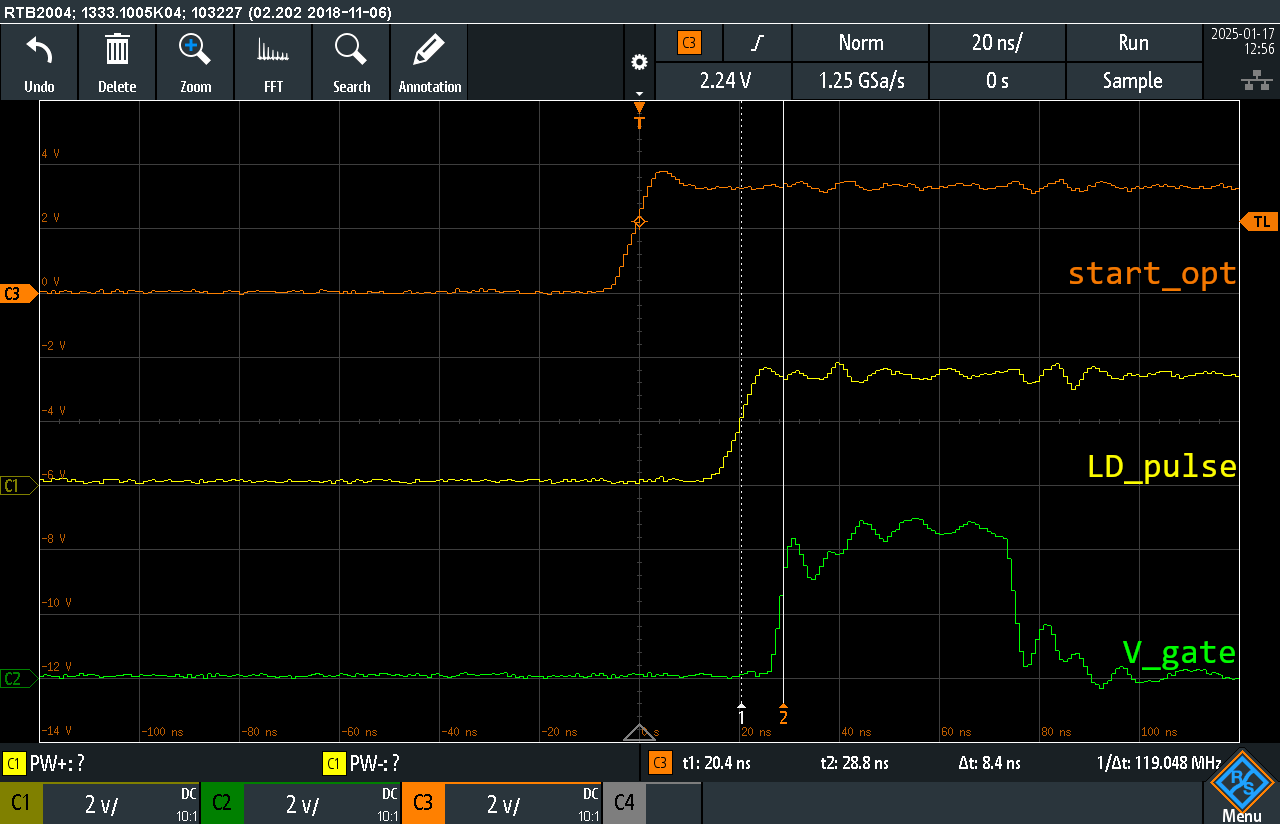
\includegraphics[width=\textwidth]{../graphics/signalpfad_sender_startopt_ldpulse_fetgate.png}
      \caption{Measurement of the signal path sender: \lstinline|start_op|, \lstinline|LD_pulse|, FET gate}\label{fig:signalpfad_sender_startopt_ldpulse_fetgate}
\end{figure}

The measured delay time of 20.4 ns (20.8 ns corresponds to one clock cycle at 48 MHz) between
\lstinline|start_op| and \lstinline|LD_pulse| was deliberately inserted to ensure that the minimum measurement duration
of 12 ns \cite{ti2016tdc7200_datasheet} in mode 1 is always guaranteed.

The measured delay time of 8.4 ns between \lstinline|LD_pulse| and the FET gate (this corresponds to the output
of the gate driver \lstinline|IC22|) is small and shows a steep edge.

Figure~\ref{fig:signalpfad_sender_ld_strom} shows the current through the laser diode (\lstinline|LD1| in
Figure~\ref{fig:laser_driver}).

\begin{figure}[H]
      \centering
      
\includegraphics[width=\textwidth]{../graphics/signalpfad_sender_ld_strom}
      \caption{Measurement signal path sender: Current through laser diode}\label{fig:signalpfad_sender_ld_strom}
\end{figure}

The current was calculated using the formula~\ref{eq:messung_strom_ld}.

\begin{equation}\label{eq:messung_strom_ld}
      I_{LD} = \frac{V(\text{\lstinline|TP8|}) - V(\text{\lstinline|TP9|})}{R_V} = \frac{V(\text{\lstinline|TP8|}) - V(\text{\lstinline|TP9|})}{5~\Omega}
\end{equation}
\myequations{Calculation of current through laser diode}

To make the delay time visible, the signal \lstinline|LD_pulse| and the potential at the FET gate were also recorded, as
in Figure~\ref{fig:signalpfad_sender_startopt_ldpulse_fetgate}.

The measured current during transmission is approximately 174 mA.

This is considerably less than the expected current of 440 mA from formula~\ref{eq:rld65nzx1_higher_output}. This is due to
the increased diode voltage. During transmission, the voltage across the laser diode increases to approximately 4 V, while the
voltage across the drain-source of the FET is negligible. This results in the current through the diode according to the
formula~\ref{eq:strom_ld_tatsaechlich}.

\begin{equation}\label{eq:strom_ld_tatsaechlich}
      I_{LD} = \frac{5~V - V_{LD} - V_{DS}}{R_V} \approx \frac{5~V - 4~V}{5~\Omega} \approx 200~mA
\end{equation}
\myequations{Calculation of current through laser diode (actual)}

\subsubsection{ToF measurements via mirror}\label{sec:measurements_mirror}

To ensure that the photodiode receives the strongest possible signal, a mirror was used instead of a wall for these
measurements. The setup is shown in Figure~\ref{fig:spiegel_setup}.

\begin{figure}[H]
      \centering
      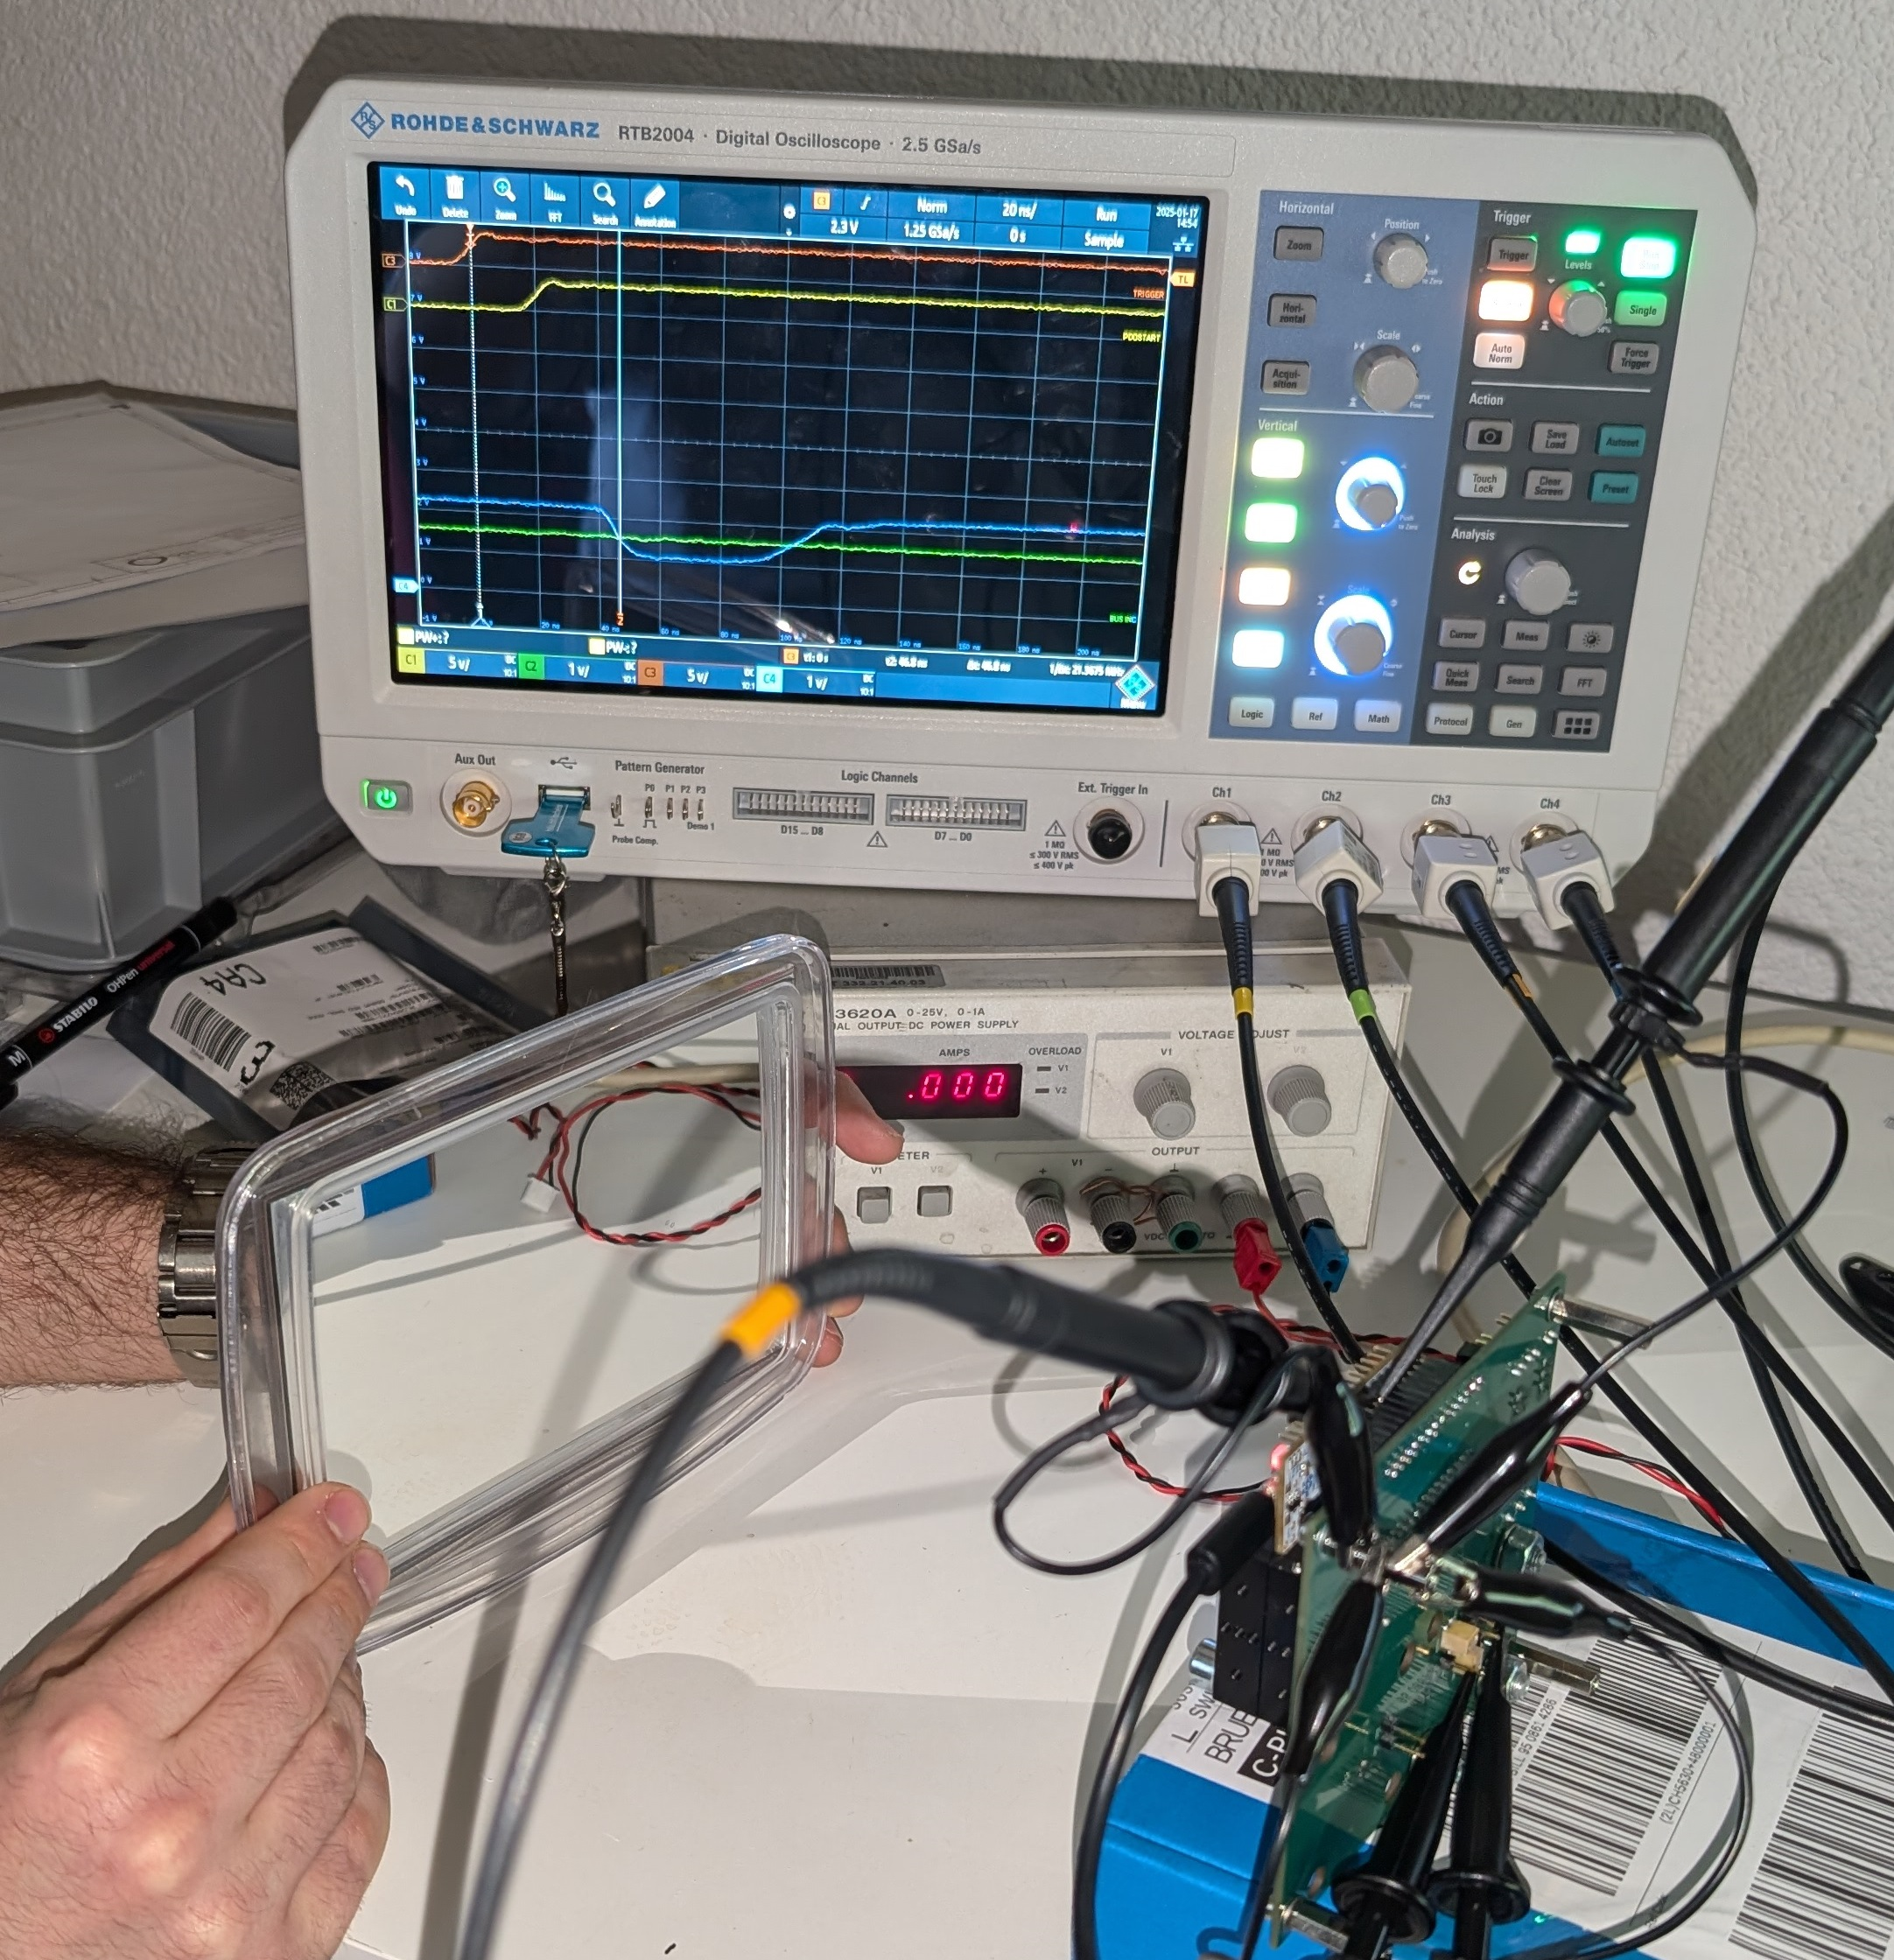
\includegraphics[width=0.6\textwidth]{../graphics/spiegel_setup.jpg}
      \caption{Measurement setup with mirror}\label{fig:spiegel_setup}
\end{figure}

According to the data sheet, the laser diode has a non-ideal point-shaped radiation pattern, see
Figure~\ref{fig:laser_abstrahl_charakteristik}.

\begin{figure}[H]
      \centering
      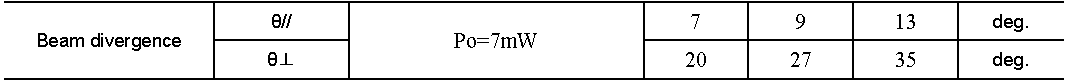
\includegraphics[width=0.8\textwidth]{../graphics/laser_abstrahl_charakteristik.pdf}
      \caption[Laser beam pattern]{Laser beam pattern \cite{rohm2019rld65nzx1_datasheet}}\label{fig:laser_abstrahl_charakteristik}
\end{figure}

It has been noticed that with the chosen \acrshort{pcb} layout, the orientation of the laser diode for a mirror
measurement. The wider beam angle is perpendicular to the line between the laser and photodiode. See
Figure~\ref{fig:laser_ausrichtung}.

\begin{figure}[H]
      \centering
      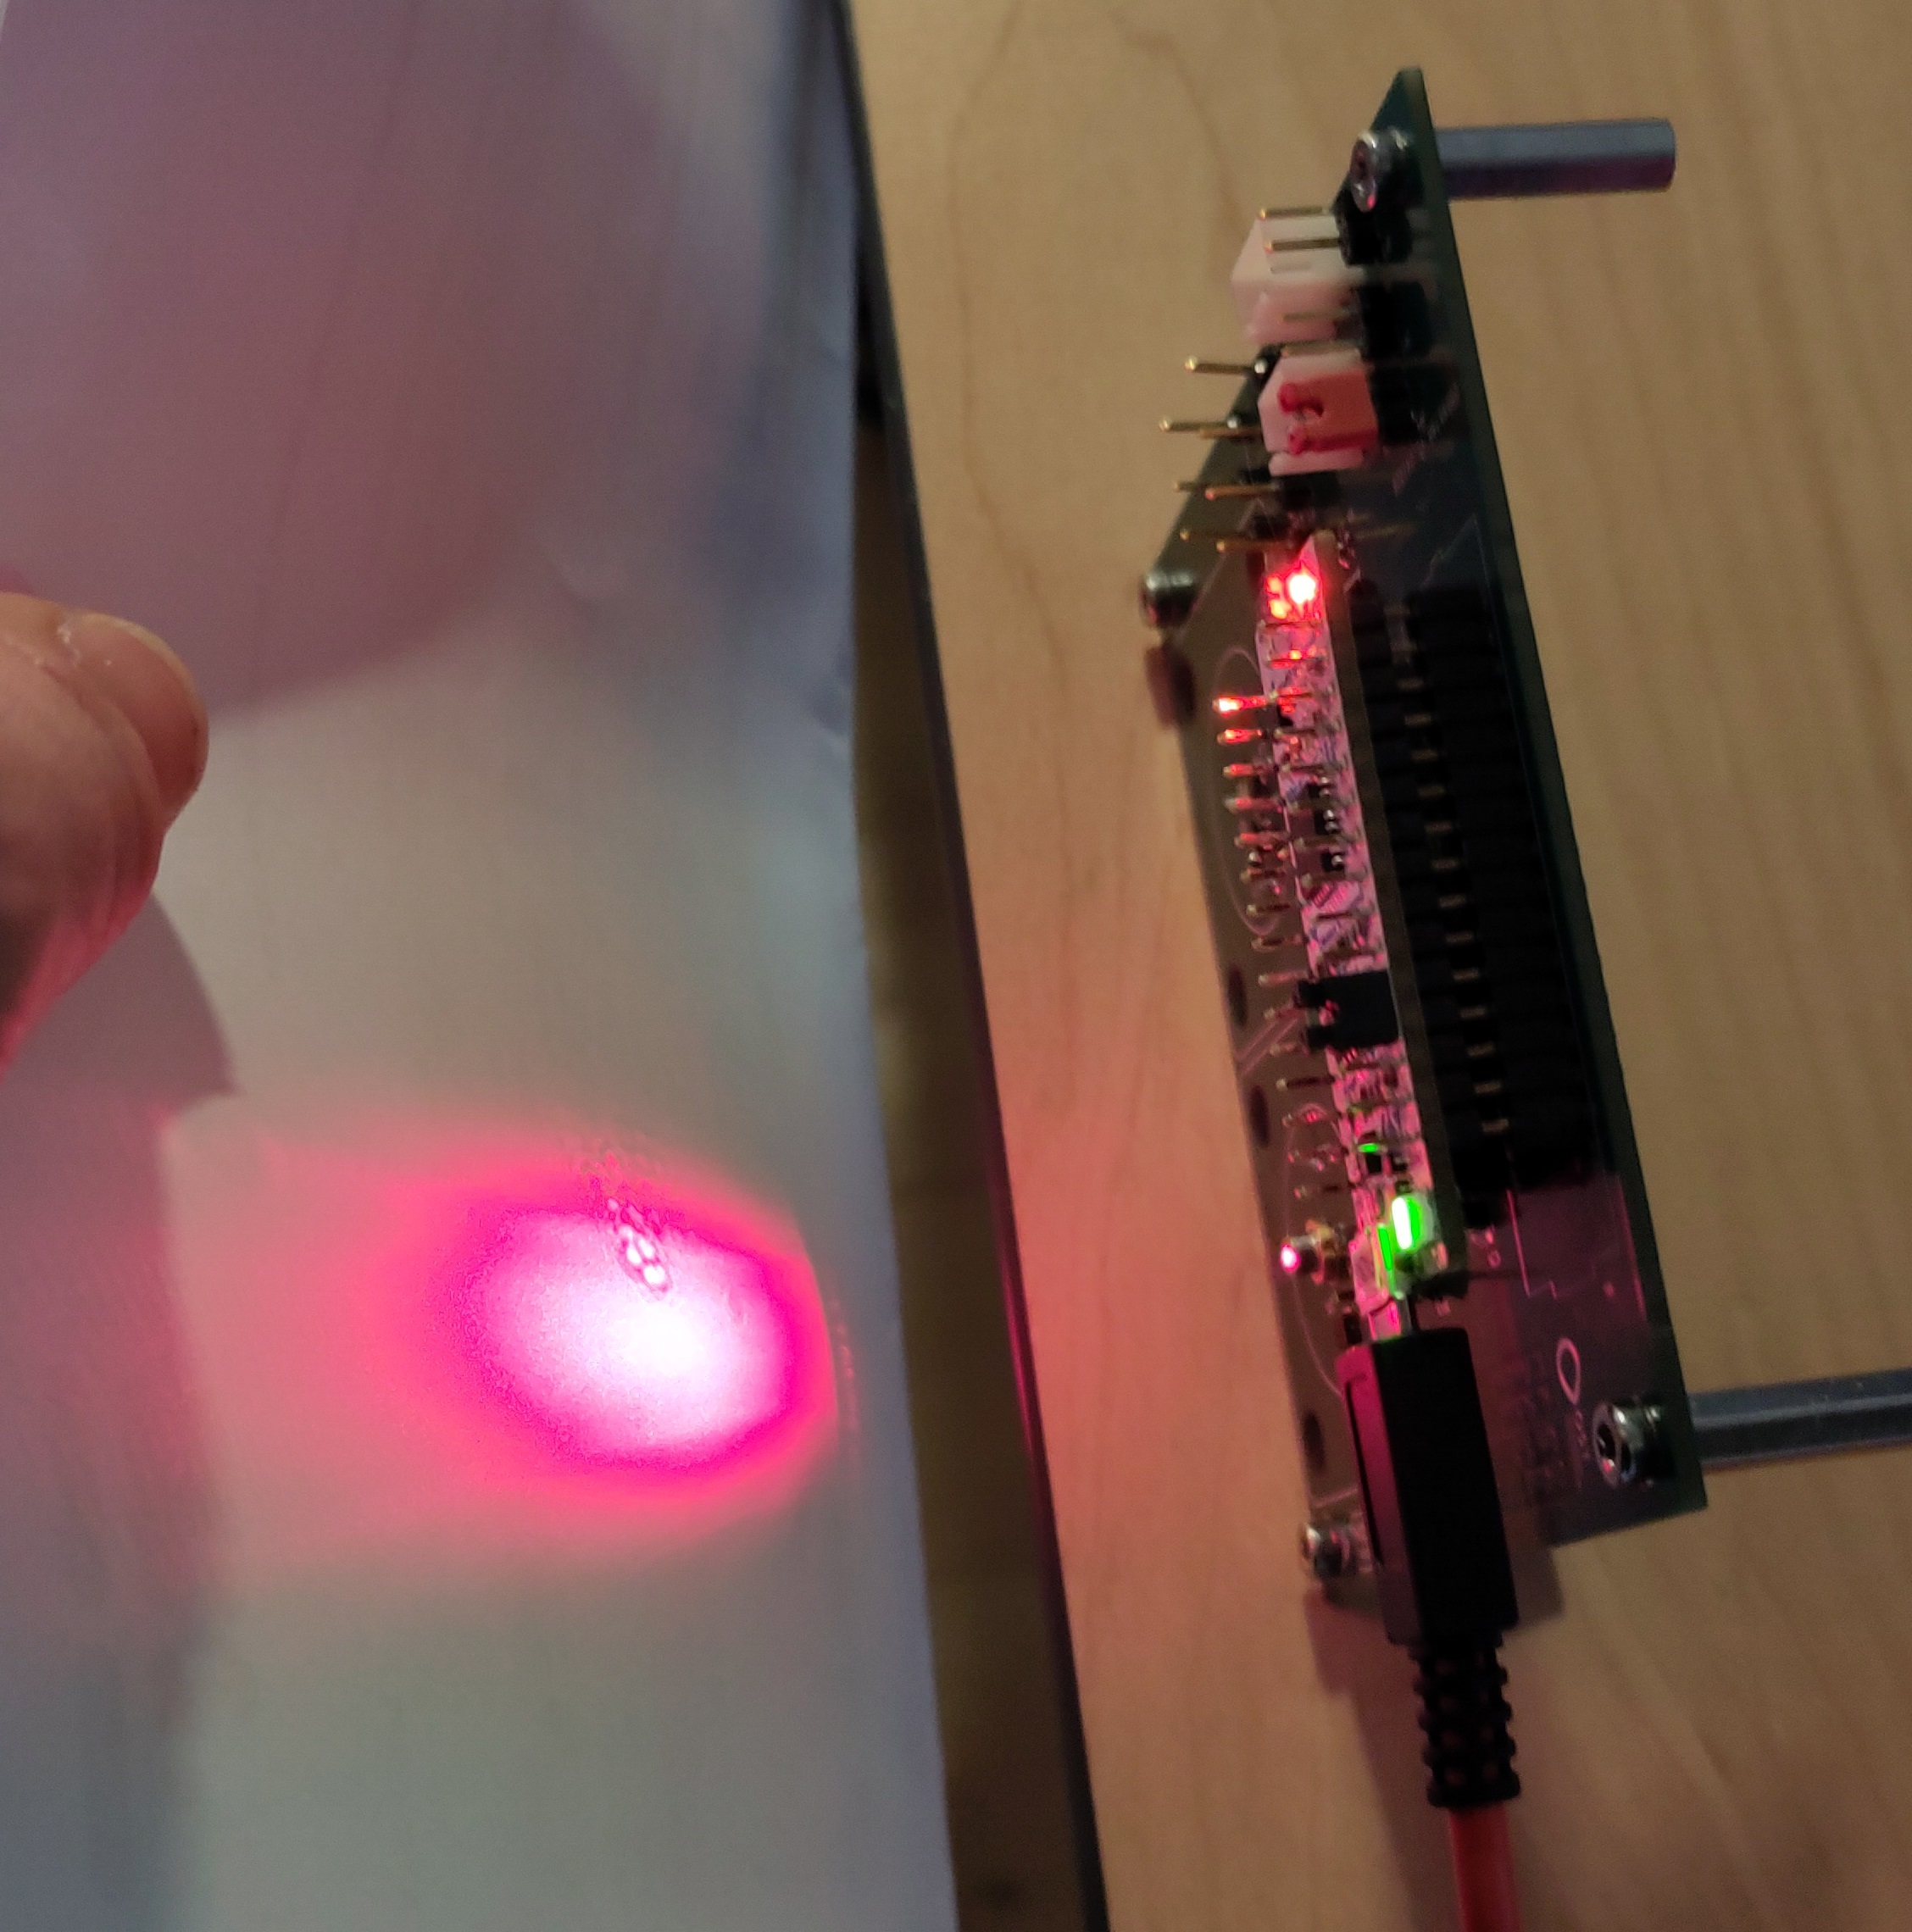
\includegraphics[width=0.6\textwidth]{../graphics/laser_ausrichtung.jpg}
      \caption{Laser alignment}\label{fig:laser_ausrichtung}
\end{figure}

The laser diode was therefore manually rotated by $90\degree$, as shown in Figure~\ref{fig:laser_ausrichtung_angepasst}.

\begin{figure}[H]
      \centering
      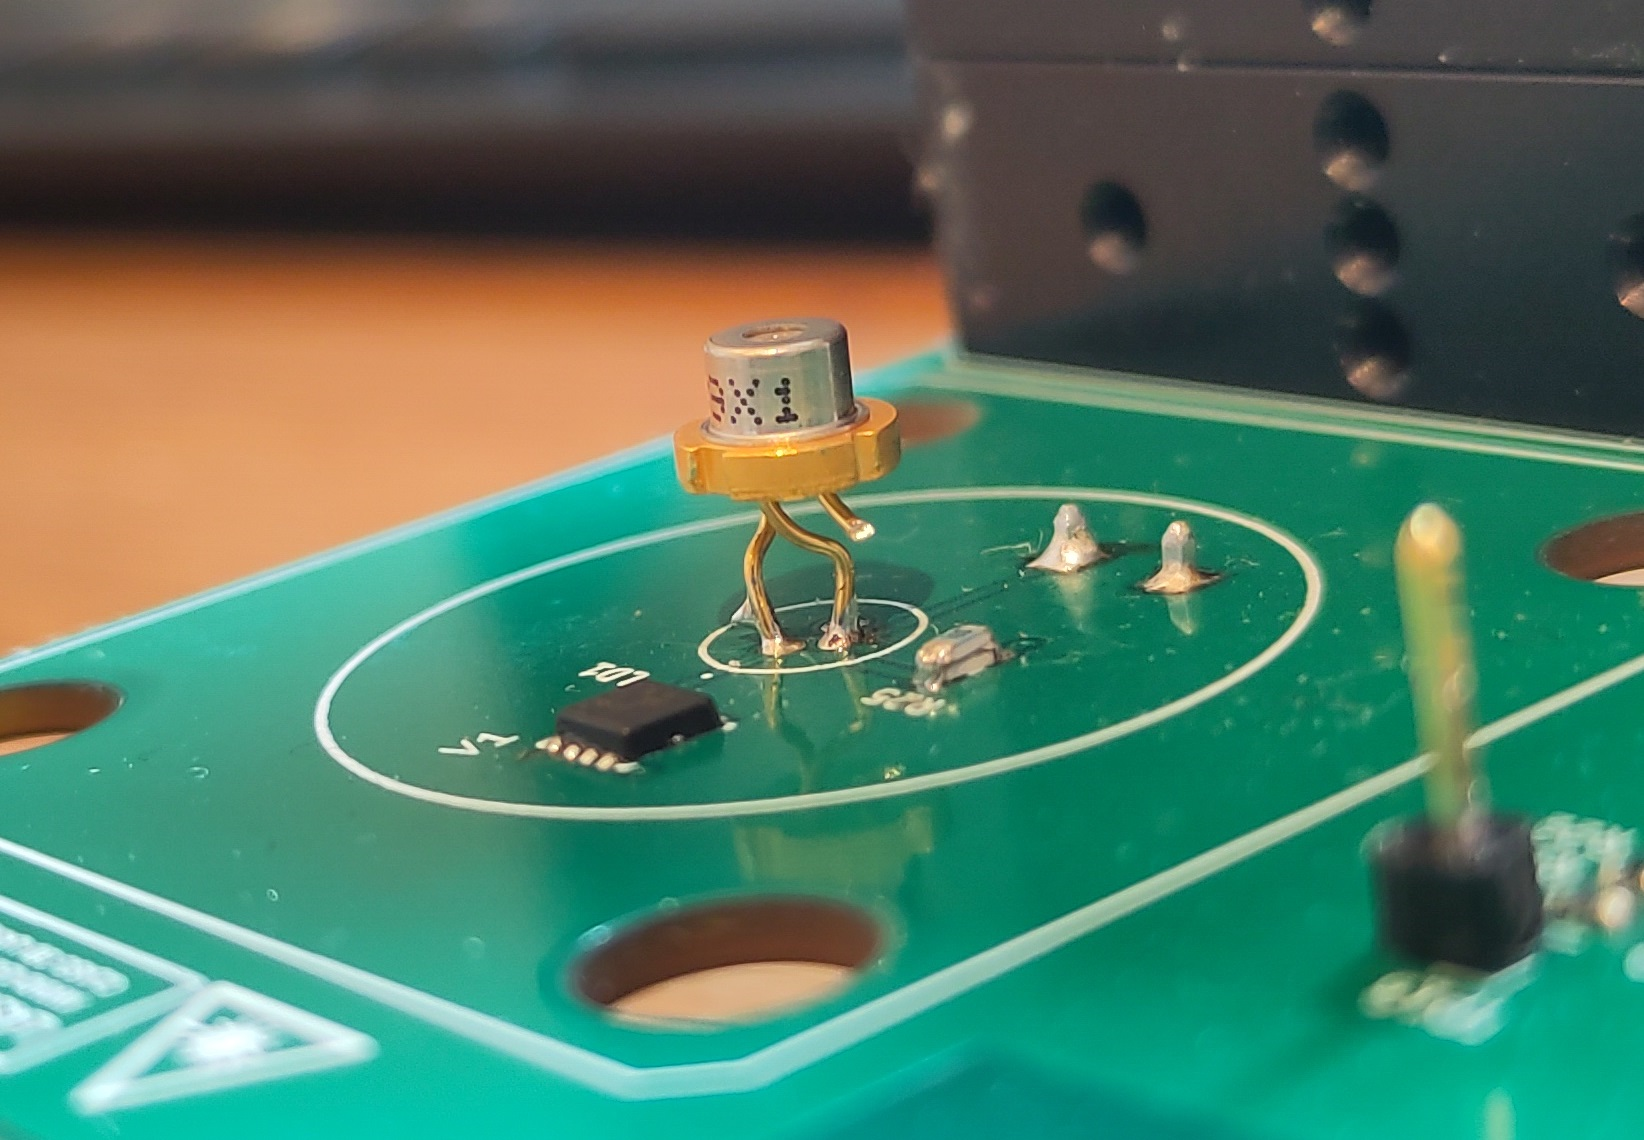
\includegraphics[width=0.6\textwidth]{../graphics/laser_ausrichtung_angepasst.jpg}
      \caption{Laser alignment adjusted}\label{fig:laser_ausrichtung_angepasst}
\end{figure}

The \acrshort{dso} diagram of an initial mirror measurement at a distance of approx. 20 cm from the mirror is shown in
Figure~\ref{fig:spiegel_initial}. It shows the output of the transimpedance amplifier. In addition, to see the delay
time, the \acrshort{mcu} signals \lstinline|start_op| and \lstinline|LD_pulse| as well as the voltage potential at the
gate of the FET.

\begin{figure}[H]
      \centering
      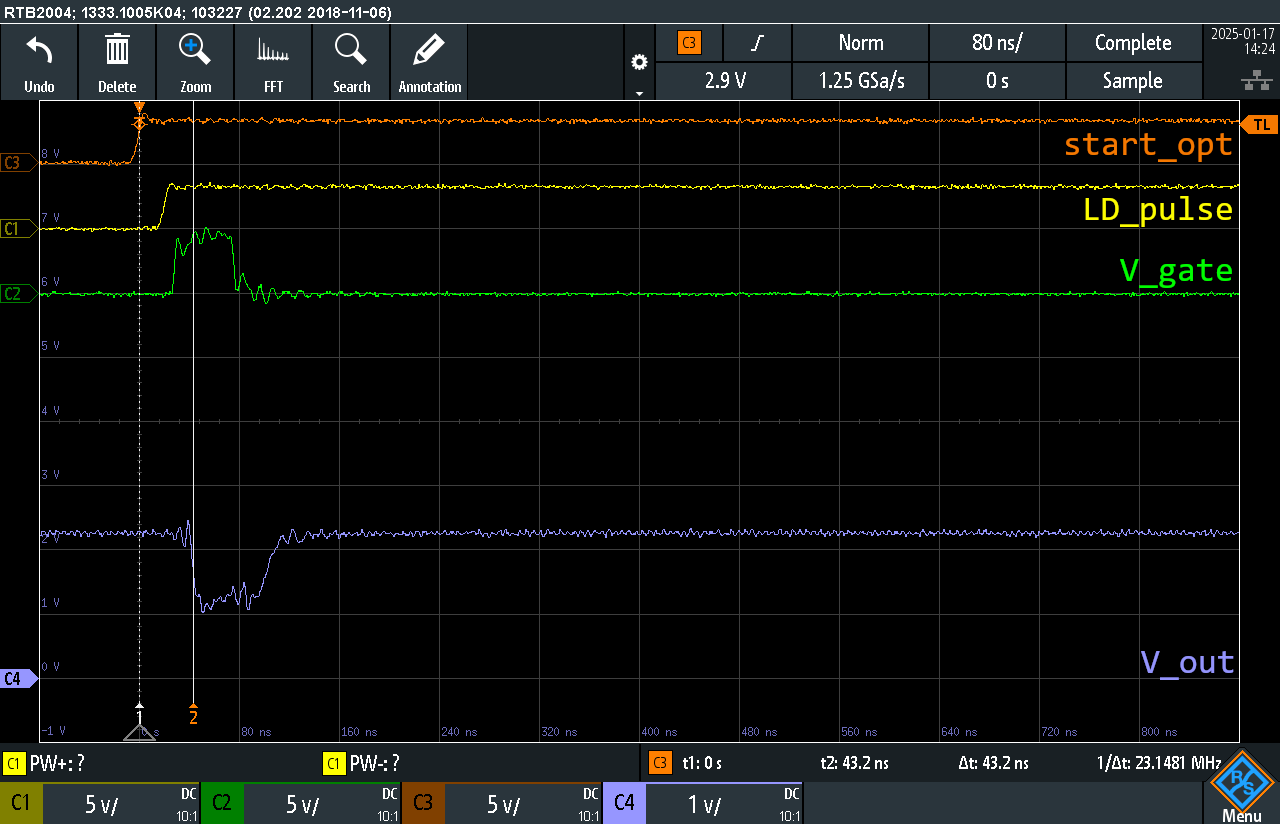
\includegraphics[width=\textwidth]{../graphics/spiegel_initial.png}
      \caption{Initial mirror measurement with \acrshort{dso}}\label{fig:spiegel_initial}
\end{figure}

The demonstrator was used to record measurements for three different distances: 19~cm, 24~cm and 28.5~cm.

The data points recorded with the optical \acrshort{tdc} are shown in
Figure~\ref{fig:spiegel_unterschiedliche_distanzen}. Approximately 300 measurements were recorded for each distance, the list
with the data points can be found in the electronic appendix.

\begin{figure}[H]
      \centering
      \includesvg[width=0.9\textwidth]{../graphics/spiegel_unterschiedliche_distanzen.svg}
      \caption{Different distances to the mirror - plot}\label{fig:spiegel_unterschiedliche_distanzen}
\end{figure}

The arithmetic mean values and the standard deviations are listed in Table~\ref{tab:spiegel_unterschiedliche_distanzen}.

\begin{table}[H]
      \mytable
      {|l|l|l|}
      {\textbf{Distance to mirror} & \textbf{Mean value} & \textbf{Standard deviation}}
      {\distance & \mean & \stddev}
      {../tables/spiegel_unterschiedliche_distanzen.csv}
      \caption{Different distances to the mirror - statistical quantities}\label{tab:spiegel_unterschiedliche_distanzen}
\end{table}

It is noticeable that the standard deviations are relatively large. This has to do in particular with the two clusters
which can be seen in Figure~\ref{fig:spiegel_unterschiedliche_distanzen}. The cause of these clusters is unclear.
One hypothesis is that they are related to the \acrshort{dso}. It was found that connecting the has a significant
influence on the offset of the \acrshort{tdc} runtime values (approx. 10~ns). Possibly the \acrshort{dso} has a
time-dependent influence on the measurement results due to the sample and hold -- depending on whether the light pulse
hits the photodiode during the sample or hold phase. The cause of these clusters should be analyzed in more detail in a
possible follow-up work.

A change in the mirror distance of 5 cm corresponds to a length change of 10 cm.

The measurements show an average change of about 0.6 ns for this length change of 10 cm.

In formula~\ref{eq:spiegel_unterschiedliche_distanzen}, the theoretically expected runtime difference is calculated.

\begin{equation}\label{eq:spiegel_unterschiedliche_distanzen}
      \Delta ToF = \frac{\Delta L}{c} = \frac{10~cm}{3 \cdot 10^8~m/s} = 0.33~ns
\end{equation}
\myequations{Theoretically expected change in runtime}

This difference (approx. factor of 2) could have several reasons:

1.) One possible explanation is that the edge becomes less steep with increasing distance, which causes a slightly
longer runtime to be measured.

2.) Another thing that stands out in Figure~\ref{fig:spiegel_unterschiedliche_distanzen} is a time drift during the recording of
the measurement data at 24~cm and 29~cm. Figure \ref{fig:spiegel_unterschiedliche_distanzen_linear} is intended to clarify this.

\begin{figure}[H]
      \centering
      \includesvg[width=0.9\textwidth]{../graphics/spiegel_unterschiedliche_distanzen_linear.svg}
      \caption{Different distances to the mirror - plot with linear interpolation}\label{fig:spiegel_unterschiedliche_distanzen_linear}
\end{figure}

However, this time drift cannot conclusively explain the measured difference.

Note: The mirror had to be aligned very precisely and then kept very stable in order to obtain results with
relatively small standard deviation (about 1 ns).

At distances of more than 30 cm, the \acrshort{tdc} signal becomes unusable.

This is because the photodiode then receives only a small amount of light and, accordingly, generates a small
photocurrent. This leads to a smaller modulation at the output of the transimpedance amplifier. Thus, the
threshold of the comparator is no longer or only just reached.

Figures~\ref{fig:spiegel_12cm_dso_ok} and \ref{fig:spiegel_30cm_dso_nok} are intended to illustrate this.

\begin{figure}[H]
      \centering
      
\includegraphics[width=\textwidth]{../graphics/spiegel_12cm_dso_ok.png}
      \caption{\acrshort{tia} output and comparator threshold at 12 cm}\label{fig:spiegel_12cm_dso_ok}
\end{figure}

\begin{figure}[H]
      \centering
      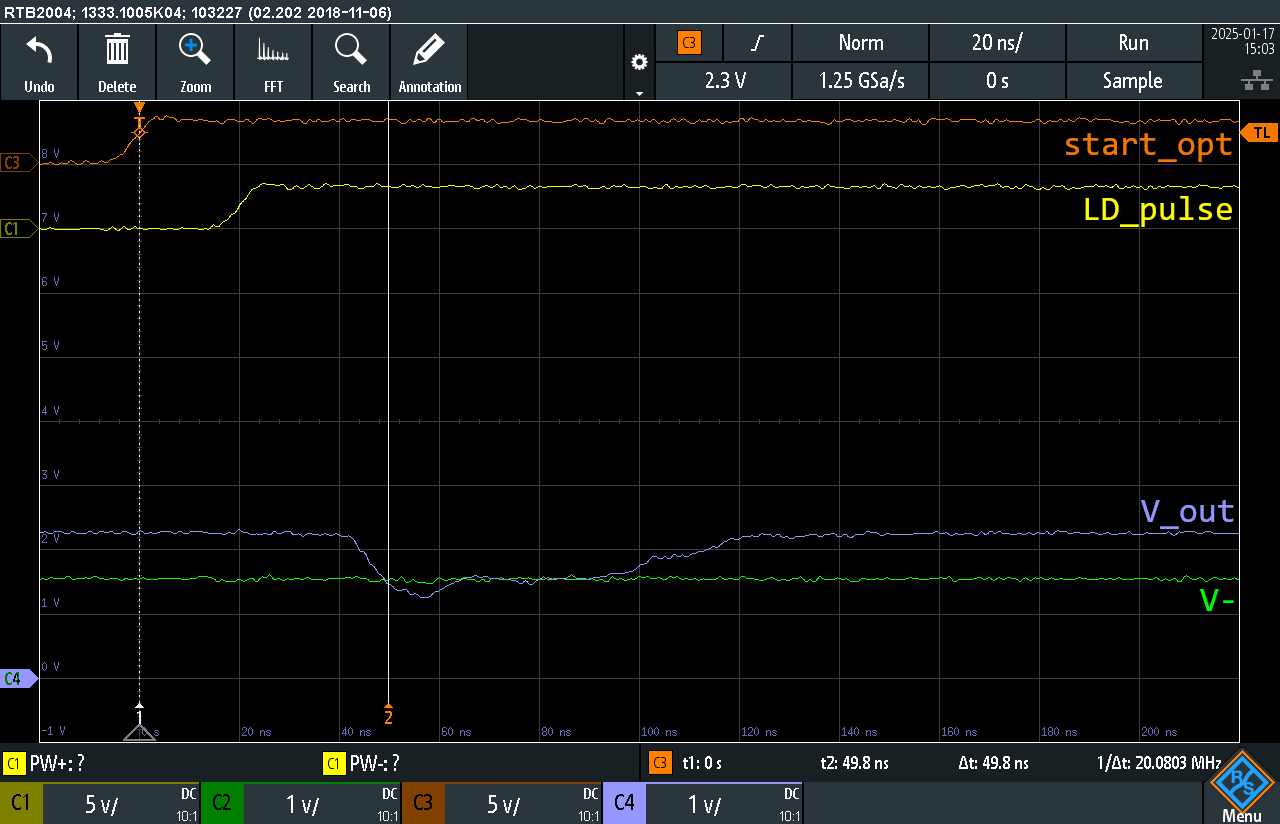
\includegraphics[width=\textwidth]{../graphics/spiegel_30cm_dso_nok.png}
      \caption{\acrshort{tia} output and comparator switching threshold at 30~cm}\label{fig:spiegel_30cm_dso_nok}
\end{figure}

The figures show, in addition to the \acrshort{mcu} signals \lstinline|start_op| and \lstinline|LD_pulse|, the output
of the transimpedance amplifier and the comparator switching threshold.

Possible improvements are listed in chapter~\ref{sec:ausblick}.

\subsubsection{ToF measurements via wall}\label{sec:messungen_wand}

Instead of the mirror used in chapter~\ref{sec:messungen_spiegel}, this chapter shows measurement results with a white
wall as a target. Distances of about 10 to 30~cm were tried.

No useful measurement results could be obtained with this setup in the short time available.

Possible improvements are listed in chapter~\ref{sec:ausblick}.
